%% Fulcrum — Topology-Aware Differential Privacy Allocation for Federated Learning
%% Target venue: IEEE Transactions on Information Forensics and Security (TIFS)
%%
%% Build: latexmk -pdf main.tex

\documentclass[letterpaper,journal]{IEEEtran}

% --- Math ---
\usepackage{amsmath,amsfonts,amssymb}
\usepackage{amsthm}

% --- Algorithms ---
\usepackage{algorithmic}
\usepackage{algorithm}

% --- Tables and figures ---
\usepackage{array}
\usepackage[caption=false,font=normalsize,labelfont=sf,textfont=sf]{subfig}
\usepackage{booktabs}
\usepackage{multirow}
\usepackage{graphicx}
\usepackage{stfloats}
\usepackage{threeparttable}

% --- Other ---
\usepackage{textcomp}
\usepackage{url}
\usepackage{verbatim}
\usepackage{xcolor}
\usepackage{orcidlink}
\usepackage{xspace}
\usepackage{enumitem}
\usepackage{tikz}
\usetikzlibrary{calc}

% --- Theorem environments (IEEEtran compatible) ---
\newtheorem{theorem}{Theorem}[section]
\newtheorem{lemma}[theorem]{Lemma}
\newtheorem{corollary}[theorem]{Corollary}
\newtheorem{proposition}[theorem]{Proposition}
\newtheorem{definition}[theorem]{Definition}

\hyphenation{op-tical net-works semi-conduc-tor IEEE-Xplore}

% --- Macros ---
\newcommand{\eg}{\textit{e.g.,}\xspace}
\newcommand{\ie}{\textit{i.e.,}\xspace}
\newcommand{\cf}{cf.\xspace}
\newcommand{\TADI}{\textsc{TADI}\xspace}
\newcommand{\Fulcrum}{\textsc{Fulcrum}\xspace}
\newcommand{\dataA}{Setting~A\xspace}
\newcommand{\dataB}{Setting~B\xspace}
\newcommand{\dataC}{Setting~C\xspace}
\newcommand{\KL}{D_{\mathrm{KL}}}
\newcommand{\RDP}{\mathrm{RDP}}
\newcommand{\Var}{\mathrm{Var}}
\newcommand{\Adv}{\mathcal{A}}
\newcommand{\Cs}{\mathcal{C}_{s}}
\newcommand{\Dset}{\mathcal{D}}
\newcommand{\TOPO}{\mathcal{G}}
\newcommand{\OBS}{\mathcal{O}}
\newcommand{\KNW}{\mathcal{K}}
\newcommand{\FAM}{\mathcal{F}}
\newcommand{\Tmax}{T_{\max}}
\newcommand{\eps}{\varepsilon}
\newcommand{\PLACE}[1]{\textcolor{red!75!black}{\textbf{[#1]}}}

\begin{document}

\title{Topology-Aware Differential Privacy in Federated Learning}

\author{Murtaza~Rangwala\orcidlink{0009-0003-4578-8671},~\IEEEmembership{Member,~IEEE,}
        Richard~O.~Sinnott\orcidlink{0000-0001-5998-222X},~\IEEEmembership{}
        and~Rajkumar~Buyya\orcidlink{0000-0001-9754-6496},~\IEEEmembership{Fellow,~IEEE}
\\
\IEEEcompsocitemizethanks{
  \IEEEcompsocthanksitem Murtaza Rangwala, Richard O. Sinnott and Rajkumar Buyya are with the Quantum Cloud Computing and Distributed Systems (qCLOUDS) Lab, School of Computing and Information Systems, The University of Melbourne, Australia.
  Email: rangwalam@unimelb.edu.au, \{rsinnott, rbuyya\}@unimelb.edu.au
}
}

\maketitle

% =============================================================================
% ABSTRACT
% =============================================================================
\begin{abstract}
Will be finalized in the end.
\end{abstract}

\begin{IEEEkeywords}
Federated Learning, Differential Privacy, Network Topology,
Distributional Inference
\end{IEEEkeywords}

% =============================================================================
% 1. INTRODUCTION
% =============================================================================
\section{Introduction}
\label{sec:intro}

Federated learning (FL) enables collaborative model training across
distributed participants without centralising raw data. Clients share
only model updates, so sensitive records, whether patient files,
clinical measurements, or proprietary assay results, remain local to
each participant~\cite{sheller2020medicine,dayan2021covid,melloddy2024,bonawitz2019sysml}.
The privacy premise is that an adversary observing these updates
learns little about the underlying data.

Considerable work has shown this premise requires active enforcement.
Gradient inversion attacks can reconstruct individual training samples
from unprotected gradient observations~\cite{zhu2019dlg,geiping2020inverting},
membership inference attacks can determine whether a specific record
participated in training~\cite{shokri2017membership}, and property
inference attacks can recover distributional attributes of a client's
local dataset from the joint update sequence~\cite{melis2019exploiting}.
The standard defense against this class of content-level leakage is
differentially private SGD (DP-SGD)~\cite{abadi2016dpsgd}, which
clips and noise-perturbs each client's gradient before transmission,
bounding the influence of any individual training record on the
observable update. Its federated instantiation, DP-FedAvg~\cite{mcmahan2018dpfedavg},
applies this mechanism within the FedAvg aggregation protocol, and
Renyi differential privacy (RDP)~\cite{mironov2017rdp} provides the
tightest known composition accounting for the cumulative privacy cost
across training rounds.

These defenses operate on the content of updates. They do not account
for what the communication topology of the federation itself reveals.
Real deployments are structurally heterogeneous: hospital consortia
route updates through regional aggregators before reaching a central
server~\cite{liu2020hierarchical,abad2020icassp}, industrial
deployments employ peer-to-peer gossip
protocols~\cite{roy2019braintorrent,hegedus2021decentralized}, and
various DAG-based aggregation schemes have been proposed for
operational scalability~\cite{beilharz2021dag}. Topology is treated
as a performance design parameter~\cite{wang2021fieldguide}, and its
privacy implications have received little systematic attention. A
passive adversary who knows the communication topology and
organisational structure of the federation, and who observes
per-round parameter updates, has access to two information channels
that DP-SGD leaves entirely unaddressed: the structural position of
each client in the communication graph, and the organisational
membership encoded by the deployment. Together, these channels may expose each client's sensitive-class concentration even when the parameter channel is effectively noise-saturated.

This paper characterises that leakage formally and derives a
principled defense, both grounded in the same threat model. We introduce \TADI (Topology-Aware Distributional Inference), a shadow-trained regressor~\cite{shokri2017membership} that estimates each client's sensitive-class concentration from observed parameter
sequences, structural graph features, and organisational labels. Four
channel ablations isolate the marginal information contributed by each
input channel, and a constant-mean calibration baseline ensures the
attack registers no advantage under the IID-null condition, where no
topology-data correlation exists.

The attack analysis exposes a fundamental decomposition. The
information an adversary can extract about a client's data separates
additively into a \textit{mechanism term}, which is a function of the client's
DP-SGD noise and shrinks as that noise increases, and a
\textit{prior-coupling term}, which reflects the client's structural position
within the federation and is not reducible by any per-client noise
allocation. Standard DP-SGD ignores this asymmetry by applying a
uniform noise multiplier across all clients, which is suboptimal
whenever the federation topology is asymmetric. We formalise this
observation and derive \Fulcrum, a closed-form balanced min-max
optimal noise allocation that, under a fixed utility budget, strictly
dominates uniform DP-SGD whenever structural-leverage scores are
non-uniform across clients. When the topology is symmetric and
leverage scores are equal, the allocation degenerates to
uniform DP-SGD, so it can be adopted unconditionally without penalty.\medskip

\noindent The key contributions of this paper are:
\begin{enumerate}[leftmargin=*,topsep=2pt,itemsep=2pt]
\item A formal threat model for topology-conditional distributional
  inference against DP-protected FL, with calibration loss and attack
  lift over a constant-mean baseline as the primary per-client
  metrics (Section~\ref{sec:threat}).
\item The \TADI attack with four channel ablations and a constant-mean
baseline comparator, providing the first per-channel decomposition
of topology-conditional leakage in DP-FL
(Section~\ref{sec:attack}).
\item An additive per-client mutual-information bound
  (Theorem~\ref{thm:per-client}) and the closed-form balanced min-max
  noise allocation \Fulcrum (Theorem~\ref{thm:allocation}), with three
  principled leverage proxies covering the hierarchical, decentralised,
  and cross-silo deployment regimes (Section~\ref{sec:defense}).
\item End-to-end empirical validation on Fed-ISIC2019~\cite{flamby2022},
  Fed-Heart-Disease~\cite{flamby2022}, and synthetic CIFAR-10~\cite{krizhevsky2009cifar} with parametric
  topology-data coupling (Section~\ref{sec:experiments}). \Fulcrum
  strictly dominates uniform DP-SGD on the privacy bound at every
  tested budget and observation window, with no measurable cost to
  model utility. The parameter channel is bounded by DP-SGD across
  all settings, the prior-coupling channel is empirically attained
  when shadow and target priors match, and the bound is conservative
  in a deployment-favourable direction on real cross-silo deployments.
\end{enumerate}

% =============================================================================
% 2. RELATED WORK
% =============================================================================
\section{Related Work}
\label{sec:related}

We position our work along three axes: privacy attacks against FL,
privacy mechanisms for FL, and the largely separate literature on
topology in FL. The gap our work fills, namely topology-conditional
distributional inference under DP with a defense paired by construction,
sits at the intersection of all three and, to our knowledge, has
not been addressed.

\subsection{Privacy Attacks Against Federated Learning}
\label{sec:related-attacks}

Two attack families dominate the literature, both content-oriented.
The first, \textit{gradient inversion}, reconstructs training samples
by optimising dummy inputs to match observed gradients. Zhu et~al.~\cite{zhu2019dlg}
introduced Deep Leakage from Gradients (DLG), which recovers
pixel-accurate images from per-batch gradients in the absence of
noise. Zhao et~al.~\cite{zhao2020idlg} improved upon this with iDLG,
which analytically extracts ground-truth labels before optimisation,
and Geiping et~al.~\cite{geiping2020inverting} subsequently
demonstrated that magnitude-invariant formulations can recover images
even from federated-averaging updates covering multiple local steps.
Yin et~al.~\cite{yin2021gradinversion} further showed that
high-resolution reconstruction remains feasible even with batch sizes
larger than those assumed by earlier work. This attack family degrades
sharply under DP-SGD because gradient clipping and Gaussian
perturbation destroy the high-frequency signal required for
pixel-level reconstruction~\cite{fowl2022robbing}. We treat gradient inversion as a
complementary threat relevant primarily when DP noise is weak; it is
outside the scope of our empirical evaluation.

The second family, \textit{inference attacks}, targets distributional
or membership properties rather than per-sample reconstruction.
Shokri et~al.~\cite{shokri2017membership} established the
shadow-model paradigm for membership inference, in which the
adversary trains an attack model on shadow datasets where membership
is known and applies it to the target. Nasr et~al.~\cite{nasr2019comprehensive} extended this paradigm to
the federated setting, demonstrating that a malicious participant or
aggregator can mount membership inference attacks by exploiting
gradient updates during training. Melis
et~al.~\cite{melis2019exploiting} showed that joint update sequences
leak unintended distributional properties of client datasets. Our
\TADI attack builds on this shadow-training framework but differs in
two respects: it targets a per-client distributional quantity, namely
the fraction of each client's data belonging to a sensitive class,
rather than membership, and it explicitly decomposes its information
sources into parameter, structural-position, and organisational-label
channels. To our knowledge, no prior attack isolates or quantifies
the contribution of these structural channels.

\subsection{Privacy Mechanisms for Federated Learning}
\label{sec:related-defense}

The dominant defense against content-level leakage in federated
learning is differential privacy applied at the client. Abadi
et~al.~\cite{abadi2016dpsgd} introduced DP-SGD, which clips
per-record gradients and adds calibrated Gaussian noise before
transmission. McMahan et~al.~\cite{mcmahan2018dpfedavg} instantiated
this mechanism within federated averaging as DP-FedAvg and demonstrated
its viability for production-scale next-word prediction. Wei
et~al.~\cite{wei2020nbafl} provided the first comprehensive convergence
analysis of DP-FL via the noising-before-aggregation framework, which
we adapt for our utility analysis (Proposition~\ref{prop:utility}).
Privacy accounting across training rounds is performed via Renyi
differential privacy (RDP)~\cite{mironov2017rdp}, a moment-based
composition framework that tracks cumulative privacy cost more tightly
than classical bounds. Subsampling amplification~\cite{wang2019subsampled}
extends this accounting to the Poisson-batched setting that DP-SGD
requires, where each client samples a random subset of its data per
round. The mutual-information (MI) characterisation of DP by Cuff and
Yu~\cite{cuff2016mi} and its tighter conversions between RDP and other
variants~\cite{asoodeh2021variants} provide the machinery we use to
derive the per-client MI bound of Theorem~\ref{thm:per-client}.

Beyond noise-based mechanisms, a complementary cryptographic defense
exists in the form of secure aggregation. Bonawitz
et~al.~\cite{bonawitz2017secagg} proposed a protocol that masks
individual client updates so that only their aggregate is visible to
the server. Combined with DP, secure aggregation reduces the
adversary's effective observation to neighbourhood-aggregated updates
rather than per-client ones, weakening \TADI's parameter channel
without addressing the structural and organisational channels.
\Fulcrum's allocation is compatible with secure aggregation as a
complementary defense; we discuss the implications in Section~\ref{sec:discussion} and
leave a full empirical evaluation under secure aggregation to future work.

A separate line of work permits per-individual privacy budgets driven
by user preferences, rather than a uniform budget applied across all
clients. Jorgensen et~al.~\cite{jorgensen2015personalized} introduced
personalised differential privacy for sample-release queries, and
subsequent work has extended this to ML training. Our setting is
distinct: the asymmetry that motivates per-client noise allocation is
structural, arising from topology and organisational position, rather
than preferential, and the allocation is derived from a worst-case MI
bound rather than from declared user preferences. The two lines are
complementary, and an integrated allocation combining structural
leverage with per-user preferences is a natural direction that falls outside the scope of this work.

What none of these mechanisms address is which clients should receive
how much noise when the topology breaks symmetry. Existing
implementations apply a uniform noise multiplier across all clients,
implicitly assuming a symmetric topology. Our defense generalises
this: when the topology is symmetric, the allocation reduces to
uniform DP-SGD; when it is not, the allocation balances the
per-client privacy bound across the asymmetric leverage profile.

\subsection{Topology in Federated Learning}
\label{sec:related-topology}

As discussed in Section~\ref{sec:intro}, topology-aware FL has been
studied primarily as a performance and scalability question. The
earliest cross-device benchmark suite, LEAF~\cite{leaf2018},
demonstrated that natural client-partitioned datasets exhibit
substantial heterogeneity but did not consider topology beyond the
implicit star aggregator. Hierarchical FL~\cite{liu2020hierarchical,abad2020icassp}
introduced edge aggregators between clients and the cloud to reduce
communication cost. Decentralised gossip-based
schemes~\cite{roy2019braintorrent,hegedus2021decentralized} eliminate
the central aggregator entirely, and Beilharz
et~al.~\cite{beilharz2021dag} proposed a DAG-based extension for
further operational flexibility. Briggs
et~al.~\cite{briggs2020hierarchical} cluster clients by local-update
similarity to address non-IID data, producing a hierarchical training
structure that incidentally encodes data similarity. The field guide
survey by Wang et~al.~\cite{wang2021fieldguide} documents topology
choice as one of the canonical decisions in FL system design but
treats it as orthogonal to privacy.

The privacy literature has largely assumed away topology. Threat
models almost universally assume a star configuration with a single
semi-honest aggregator, and the attacker's view, when explicitly
modelled, consists of per-client gradients without structural
metadata. This assumption is reasonable for cross-device deployments
where every client is interchangeable, but it breaks down in
cross-silo healthcare~\cite{flamby2022,sheller2020medicine,dayan2021covid},
multi-organisation industry consortia~\cite{melloddy2024}, and any
deployment that uses hierarchical or decentralised aggregation for
operational reasons.

The closest work to our attack contribution is Feng
et~al.~\cite{feng2025topology}, who demonstrated that the
communication topology of a decentralised FL system can itself be
inferred from model behaviour alone, establishing topology as a
target of inference attacks. Our threat model is complementary but
distinct: we assume the topology is known to the adversary and study
how structural position and organisational membership function as
information channels for inferring sensitive properties of client
data, rather than treating the topology as a quantity to be
reconstructed.

\begin{figure}[t]
\centering
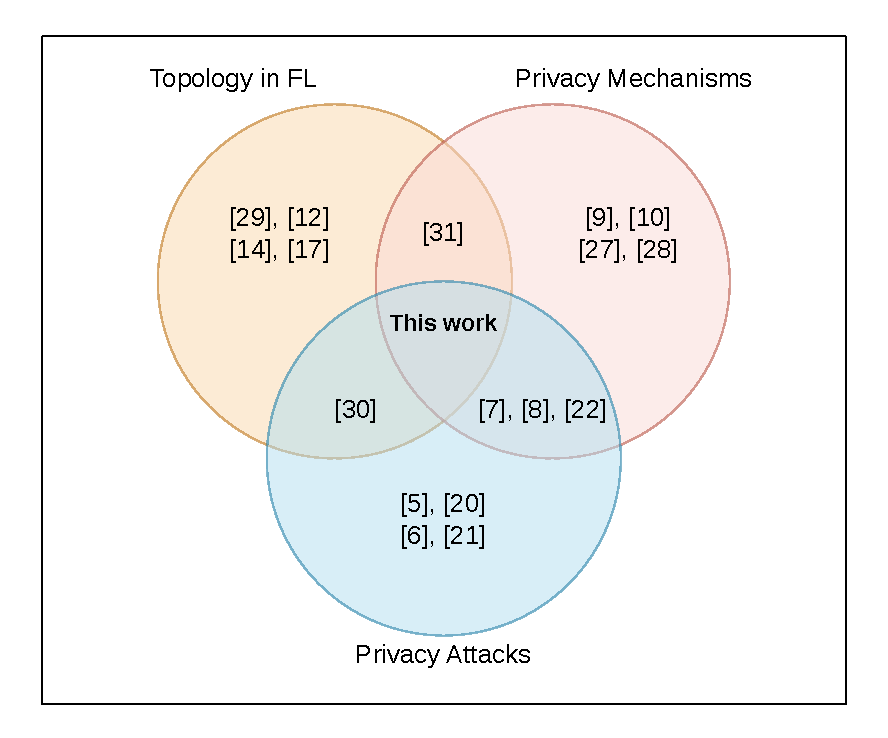
\includegraphics[width=\columnwidth]{figures/positioning.pdf}
\caption{Positioning of this work relative to the three bodies of
literature it spans. Prior work addresses at most two of the three
axes; this paper is the first to operate at their intersection.}
\label{fig:positioning}
\end{figure}

No prior work treats topology as a known information channel that an
adversary can exploit to infer sensitive data properties, nor derives
a defense that accounts for the resulting structural asymmetry. We are
the first to define a per-client distributional inference attack with
explicit channel ablations isolating parameter, structural, and
organisational information; prove an additive per-client MI bound
separating a controllable mechanism term from an uncontrollable
prior-coupling floor; and derive a closed-form noise allocation that
strictly improves on uniform DP-SGD whenever the topology breaks
leverage symmetry. Figure~\ref{fig:positioning} summarises this
positioning relative to the three bodies of literature surveyed above.

% =============================================================================
% 3. SYSTEM AND THREAT MODEL
% =============================================================================
\section{System and Threat Models}
\label{sec:threat}

We consider a passive, honest-but-curious adversary against a
DP-protected federated learning system, reflecting the realistic
scenario of a curious infrastructure observer or aggregator who
follows the protocol but exploits what they can passively
observe. Active protocol manipulation, malicious aggregators, and
Sybil attacks are outside our scope and discussed in
Section~\ref{sec:discussion}. The attack and defense are grounded in
the same formal assumptions, ensuring that the defense is evaluated
against precisely the adversary it is designed to resist.

\subsection{System Model}
\label{sec:system-model}

A federation consists of $n$ clients $\mathcal{P} = \{P_1,\ldots,P_n\}$
arranged in a communication topology $\mathcal{G} = (\mathcal{P}, E)$,
where $E$ denotes the set of edges determining which pairs of clients
communicate during aggregation. Each client $P_i$ holds a local dataset $\mathcal{D}_i$ over a class set $\mathcal{C}$ of size $K = |\mathcal{C}|$, inducing a local class distribution $\Delta_i \in \Delta(\mathcal{C})$. Clients are partitioned into organisational groups by a labelling $\omega : \mathcal{P} \to [k_{\mathrm{org}}]$, where $k_{\mathrm{org}}$ is the number of distinct groups. Training proceeds for $T_{\max}$ rounds. At each round $t$, client $P_i$ applies local DP-SGD with per-client noise scale $\sigma_i$ to
produce an updated parameter vector $\theta_i^{(t)}$, which is then
transmitted to its neighbours in $\mathcal{G}$. Topologies are assumed
to be static throughout training. Client datasets are assumed to be disjoint: no two clients share
training records. This is the standard cross-silo
assumption~\cite{wang2021fieldguide}, satisfied naturally in settings
such as hospital consortia, where each site enrols distinct patients.
Aggregation follows FedAvg~\cite{mcmahan2018dpfedavg} for centralised
hierarchical settings and decentralised
gossip~\cite{hegedus2021decentralized} for peer-to-peer topologies;
both reduce to weighted averages of client parameter vectors.

\subsection{Adversarial Model}
\label{sec:adv-model}

The adversary $\mathcal{A}$ is specified by four components: knowledge
$\mathcal{K}$, observations $\mathcal{O}$, an inference goal
$\mathcal{I}$, and a set of restrictions $\mathcal{R}$.

The adversary's knowledge $\mathcal{K}$ comprises the communication
topology $\mathcal{G}$, the organisational labelling $\omega$, and all
public protocol parameters, including the DP budget $\varepsilon$, the
per-client noise schedule $\{\sigma_j\}$, the model architecture, and
the training schedule. The adversary does not know any client's local
dataset $\mathcal{D}_i$ or its induced class distribution $\Delta_i$.
We treat $\mathcal{K}$ as a configuration constant, conditioning all
probabilistic claims on it throughout.

The adversary's observations $\mathcal{O}$ consist of the full tensor
of transmitted parameter updates,
$\Theta = \{\theta_i^{(t)} : i \in [n],\, t \in [T_{\max}]\}$, together
with communication metadata. This corresponds to a passive
infrastructure observer, such as a curious cloud aggregator or a
network-level observer with access to unencrypted traffic.

The inference goal $\mathcal{I}$ is to recover, for each client $i$,
the sensitive-class concentration
\[
p_i \;=\; \Delta_i(\mathcal{C}_s) \;\in\; [0,1],
\]
where $\mathcal{C}_s \subset \mathcal{C}$ is a designated sensitive
class set. This captures either a single sensitive proportion in
binary classification tasks, or a designated rare-class proportion in
multiclass settings. Attack performance is measured by calibration
loss $L_{\text{cal}} = \frac{1}{n}\sum_i (\hat{p}_i - p_i)^2$ and
attack lift relative to the constant-mean baseline
$\bar{p} = \frac{1}{n}\sum_j p_j$, which measures whether the
adversary extracts information beyond the federation aggregate.

The restrictions $\mathcal{R}$ define an honest-but-curious adversary.
The adversary follows the protocol faithfully, cannot perturb
$\theta_i^{(t)}$ prior to observation, cannot inject training data,
cannot collude with clients, and cannot adaptively select targets.

\subsection{Independence Assumptions}
\label{sec:independence}

\noindent Two assumptions underpin the formal analysis.\medskip

\noindent\textbf{(IA1) DP-SGD noise independence.} The per-round Gaussian noise
$\xi_i^{(t)} \sim \mathcal{N}(0, \sigma_i^2 C^2 I)$ is independent
across all $(i, t)$ pairs. This is standard in the DP-SGD
literature~\cite{abadi2016dpsgd}.\medskip

\noindent\textbf{(IA2) Disjoint client datasets.} For $i \neq j$,
$\mathcal{D}_i \cap \mathcal{D}_j = \emptyset$, as established in
Section~\ref{sec:system-model}. Cross-device settings where the same
individual contributes to multiple clients would require strengthened
conditions; we flag this as a limitation in
Section~\ref{sec:discussion}.\medskip

\noindent Aggregation follows FedAvg or its hierarchical and gossip variants
and is not treated as a privacy mechanism in our threat model, since
the adversary observes per-client updates prior to aggregation. Under
secure aggregation~\cite{bonawitz2017secagg} this changes; \Fulcrum
is compatible with secure aggregation as a complementary defense, and
we discuss this in Section~\ref{sec:discussion}.

\subsection{Reference Adversaries}
\label{sec:reference-adv}

To isolate the contribution of each information channel, we define
five reference adversaries differing only in their knowledge
$\mathcal{K}$, with observations $\mathcal{O} = \Theta$ in all cases.

\begin{itemize}[topsep=2pt,itemsep=2pt,leftmargin=*]
\item $\mathcal{A}_0$ (constant-mean baseline): outputs the federation
  mean $\bar{p}$ for every client. Serves as the reference for
  computing attack lift.
\item $\mathcal{A}_1$ (parameter-only): $\mathcal{K} = \{\sigma_j\}$.
  Recovers $\hat{p}_i$ from parameter sequences alone, with no access
  to structural or organisational information. This is the
  topology-agnostic adversary of Melis et~al.~\cite{melis2019exploiting}.
\item $\mathcal{A}_2^{\text{topo}}$ (structural): $\mathcal{K} =
  \mathcal{G}$. Augments parameter sequences with structural features
  including degree, hierarchical depth, and distance to root,
  isolating the marginal information value of the communication
  topology.
\item $\mathcal{A}_2^{\text{org}}$ (organisational): $\mathcal{K} =
  \omega$. Augments parameter sequences with organisational labels,
  isolating the marginal information value of organisational
  membership.
\item $\mathcal{A}_2^{\text{full}}$ (full knowledge): $\mathcal{K} =
  (\mathcal{G}, \omega, \{\sigma_j\})$. The primary adversary of
  interest.\medskip
\end{itemize}

The topology contribution is measured as
$L_{\text{cal}}(\mathcal{A}_1) - L_{\text{cal}}(\mathcal{A}_2^{\text{full}})$,
and the marginal contributions of structure and organisational label
are obtained by comparing $\mathcal{A}_2^{\text{full}}$ against the
corresponding partial adversary. The IID-null condition arises when
the data partitioning makes $p_i$ constant across clients, in which
case every adversary's calibration loss equals $\mathrm{Var}(p)$ and
attack lift is identically zero. We use this condition as a consistency check that holds by construction throughout the empirical evaluation.

% =============================================================================
% 4. THE TADI ATTACK
% =============================================================================
\section{The \TADI Attack}
\label{sec:attack}

\TADI is a learned regressor with four channel ablations, each corresponding to a different subset of the adversary's available information. The architecture maps observable inputs to per-client sensitive-class concentration estimates; the ablations differ only in which channels of $\mathcal{K}$ and $\mathcal{O}$ are exposed to the regressor. This design serves two purposes: it provides the empirical characterisation of topology-conditional leakage, and it ensures the channel boundaries align with the decomposition required by the theoretical bound in Section~\ref{sec:defense}.

\subsection{Attack Architecture}
\label{sec:attack-arch}

Let $f_\phi : (\Theta_i, x_i) \to \hat{p}_i \in [0,1]$ denote the
adversary's regressor with learnable parameters $\phi$. The regressor
takes two classes of input, as illustrated in
Figure~\ref{fig:tadi-pipeline}.

The first is the parameter sequence
$\Theta_i = (\theta_i^{(1)}, \ldots, \theta_i^{(T_{\max})})$, from
which we extract a fixed-dimensional feature vector combining
per-round and temporal-aggregate signals. Per-round signals comprise
parameter norms $\{\|\theta_i^{(t)}\|_2\}$, layer-wise norms, and
pairwise cosine similarities to neighbouring clients' updates.
Temporal aggregates comprise the mean and standard deviation of
parameter norms across rounds, a linear trend estimate, and the
last-round parameter value.

The second is a structural and organisational feature vector
$x_i \in \mathbb{R}^k$ derived from $(\mathcal{G}, \omega)$.
Structural features comprise client $i$'s degree in $\mathcal{G}$,
its distance to the topology root, and its betweenness centrality.
The organisational label $\omega_i$ is encoded as a one-hot vector
and concatenated with the structural features. Distance to root is
defined for rooted topologies such as hierarchical FL; for
decentralised peer-to-peer topologies without a natural root, this
feature is set to zero. Betweenness centrality is precomputed from
the known topology $\mathcal{G}$ prior to training.

\begin{figure*}[t]
\centering
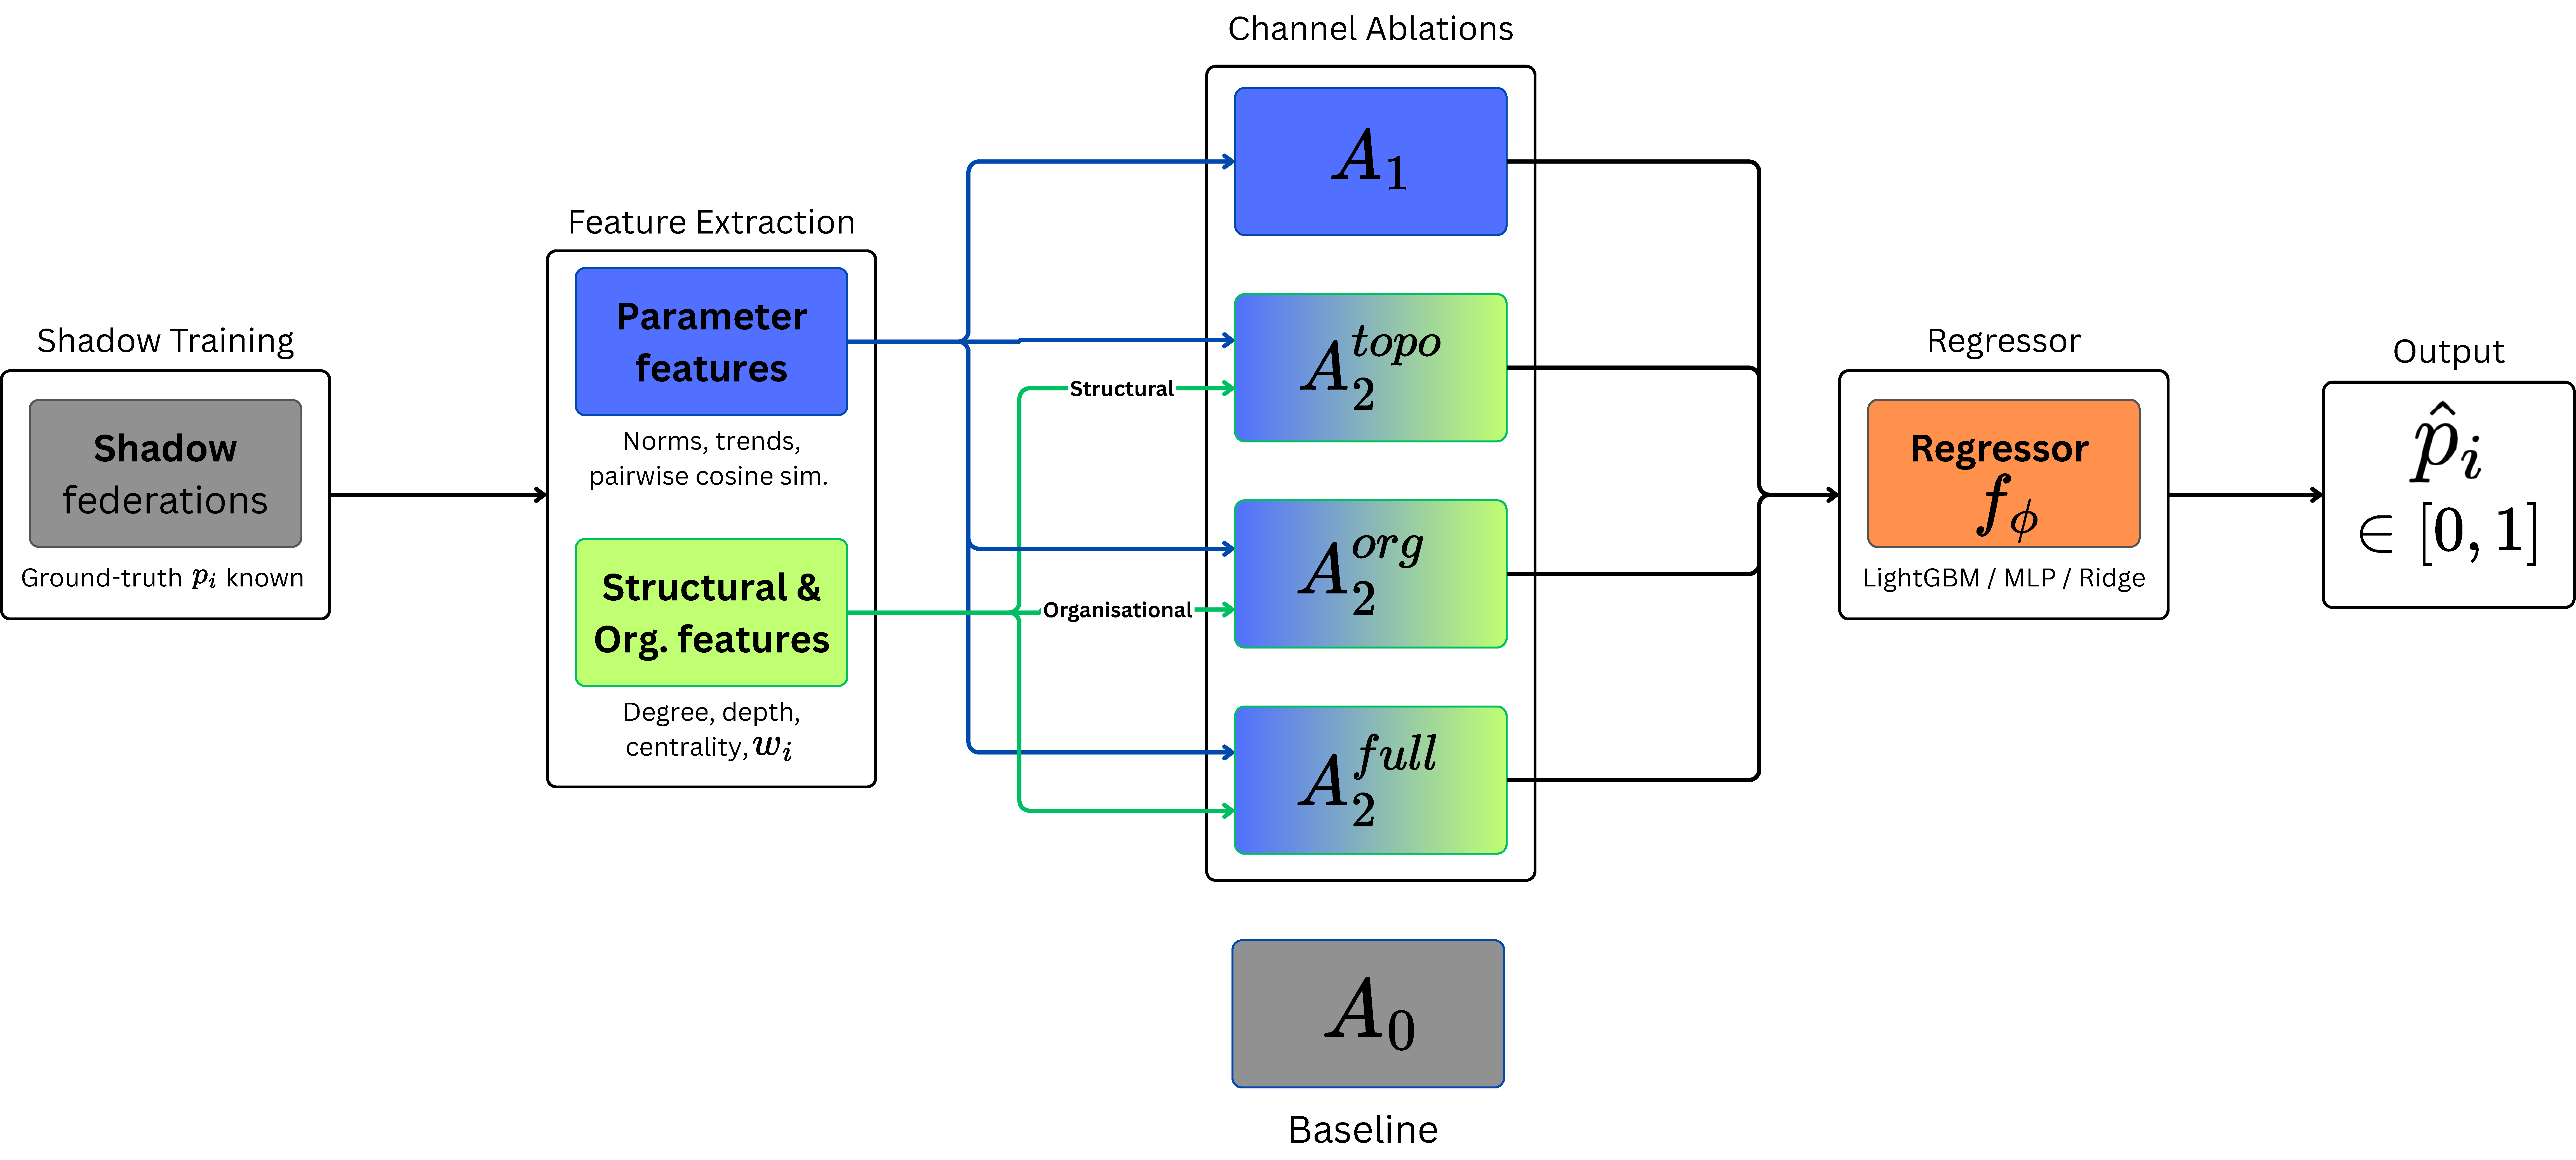
\includegraphics[width=\linewidth]{figures/tadi_pipeline.pdf}
\caption{The \TADI attack pipeline. The adversary simulates shadow
federations to harvest labelled training tuples, extracts parameter
and structural features, selects a channel subset corresponding to
one of the four ablations, and fits a regressor $f_\phi$ to estimate
the sensitive-class concentration $\hat{p}_i$ for each client.
$\mathcal{A}_0$ is the constant-mean baseline and does not correspond
to a channel ablation.}
\label{fig:tadi-pipeline}
\end{figure*}

The regressor is trained offline via the shadow-model
framework~\cite{shokri2017membership}. The adversary simulates
federations on a public proxy dataset where the ground-truth $p_i$
is known, harvests $(\Theta_i, x_i, p_i)$ tuples across many
simulated clients, and fits $f_\phi$ to minimise mean squared
calibration loss on the harvested set. At test time, $f_\phi$ is
applied to the target federation. The test-time adversary is
therefore a deterministic function of $(\mathcal{K}, \mathcal{O})$,
consistent with the threat model of Section~\ref{sec:adv-model}.

To assess robustness to the choice of model class, we instantiate
$f_\phi$ with three regressor backends: gradient-boosted trees
(\textsc{LightGBM}, the default), a small multilayer perceptron, and
ridge regression. All produce predictions clipped to $[0,1]$.

\subsection{Channel Ablations}
\label{sec:attack-channels}

The four ablations correspond to the reference adversaries of
\S\ref{sec:reference-adv}. They differ only in which features the
regressor sees:

\begin{description}[itemsep=2pt,leftmargin=*]
\item[$\Adv_1$] Parameter-only. Input: parameter features extracted from
  $\Theta_i$. Topology and organisational labels are zeroed out.
\item[$\Adv_2^{\text{topo}}$] Structural-only. Input: structural features
  from $(\TOPO,i)$, including degree, depth, and centrality. Parameter features
  zeroed.
\item[$\Adv_2^{\text{org}}$] Organisational-only. Input: one-hot
  $\omega_i$. Parameter features zeroed.
\item[$\Adv_2^{\text{full}}$] All three concatenated.
\end{description}

A separate regressor is trained per channel on the same shadow corpus.
This keeps the comparison apples-to-apples across channels: each
$\hat p_i$ is the best the regressor can do given exactly that channel's
input.

\subsection{Metric Panel}
\label{sec:attack-metrics}

Per (target run, channel) pair we compute:

\begin{description}[itemsep=2pt,leftmargin=*]
\item[Calibration loss] $L_{\text{cal}}(\hat p, p) = \frac{1}{n}\sum_i (\hat p_i - p_i)^2$.
  Primary metric. Has statistical power even at $n=4$ (Setting~B).
\item[Constant-mean baseline]
  $L_{\text{cal}}(\bar p, p) = \Var(p)$ where
  $\bar p_i \equiv \frac{1}{n}\sum_j p_j$. The trivial predictor.
\item[Attack lift]
  $L_{\text{cal}}(\bar p, p) - L_{\text{cal}}(\hat p, p)$.
  Positive iff the adversary extracts client-level information beyond
  the federation aggregate; identically zero under the IID null.
\item[Top-$k$ recovery] Fraction of true top-$k$ clients (by
  $p_i$) in the predicted top-$k$. Bounded, interpretable.
\item[AUROC] for the binary task
  $y_i = \mathbb{1}[p_i > \tau]$. Reported across all settings as a
  ranking-quality indicator; statistical power for AUROC requires
  $n \geq 20$, so quantitative significance applies primarily to
  Setting~C, with Setting~B's AUROC ($n=4$) treated as directional.
\end{description}

Statistical significance is assessed via paired bootstrap on calibration
loss across seeds, with multiple-comparison correction across the four
channels.

\subsection{Algorithmic Summary}
\label{sec:attack-algo}

\begin{algorithm}[t]
\caption{\TADI{}, full-channel variant ($\Adv_2^{\text{full}}$)}
\label{alg:tadi}
\begin{algorithmic}[1]
\REQUIRE Shadow corpus $\mathcal{S} = \{(\Theta_i, x_i, p_i)\}$,
         target observations $(\Theta^{\text{tgt}}, \TOPO, \omega, \{\sigma_j\})$,
         regressor backend $\mathcal{B}$
\ENSURE  Per-client estimates $\{\hat p_i\}$ and metric panel
\STATE Extract parameter features $\phi_{\Theta}^{(i)}$ from
       each $\Theta_i \in \mathcal{S}$
\STATE Build structural features $\phi_x^{(i)} = [\deg(i), \mathrm{depth}(i), \mathrm{cent}(i), \mathrm{onehot}(\omega_i)]$
\STATE Train $f \gets \mathcal{B}.\mathrm{fit}(
       \{[\phi_{\Theta}^{(i)}; \phi_x^{(i)}]\}, \{p_i\})$
\FOR{client $i$ in target federation}
  \STATE $\hat p_i \gets \mathrm{clip}_{[0,1]}\big( f([\phi_{\Theta}^{(\text{tgt},i)}; \phi_x^{(\text{tgt},i)}]) \big)$
\ENDFOR
\RETURN $\{\hat p_i\}$ along with $L_{\text{cal}}, L_{\text{cal}}(\bar p,p),
       \text{lift}, \mathrm{top}\text{-}k, \mathrm{AUROC}$
\end{algorithmic}
\end{algorithm}

The other three ablations replace the concatenation in line~3 with the
appropriate channel subset.

\subsection{What \TADI is and is not}
\label{sec:attack-positioning}

As a learning architecture, \TADI is shadow-trained supervised
regression on parameter and structural features; novelty lies not in
the model class but in the channel decomposition it enables. The
contribution is the empirical \emph{characterisation} that this attack
yields under DP-SGD across the four channel ablations, on FL
benchmarks, with explicit attribution of marginal information value to
parameter, structural, and organisational components. The attack also
serves as the empirical comparator against which we evaluate the
realisability of the privacy bound proved in \S\ref{sec:defense}.

\paragraph{What the channel decomposition is for.}
We use the four channels as a \emph{decomposition} of the adversary's
available information, not as a tournament of strictly ordered
attackers. The empirical questions we ask of the decomposition are:
(i) does DP-SGD effectively bound the parameter channel under the
per-client allocation, separately from any prior coupling?
(ii) which non-parameter channel (structural position or organisational
label) carries the prior-coupling signal in a given deployment?
(iii) is the prior-coupling channel's signal realisable under the
public-proxy threat model of \S\ref{sec:adv-model}, or does the
synthetic-shadow vs.\ native-target prior gap make
$\ell_i^\circ$'s supremum out of reach?

\paragraph{What we do not claim.}
A natural hypothesis is that the combined adversary $\Adv_2^{\text{full}}$
strictly dominates each single-channel ablation. The evidence in
\S\ref{sec:experiments-channels} qualifies this hypothesis on both
settings examined:

\begin{itemize}[topsep=2pt,itemsep=2pt,leftmargin=*]
\item On Setting~C (matched shadow/target prior), the org channel
  dominates the combined channel on attack lift and top-$k$ recovery
  while the combined channel marginally edges it on AUROC; the
  regressor's combined feature set picks up noise that the additional
  channels add without enough signal to overcome it on a finite
  shadow corpus.
\item On Setting~B (mismatched shadow/target prior), the combined
  channel reaches the highest AUROC of the four ($0.56$) but no
  channel achieves positive attack lift; the prior gap is empirically
  binding.
\end{itemize}

The four channels are therefore best understood as a decomposition
of information sources, with the realised-channel-dominance pattern
depending on the deployment regime and the adversary's prior
knowledge.

% =============================================================================
% 5. DEFENSE
% =============================================================================
\section{Defense: Topology-Aware DP Allocation}
\label{sec:defense}

The defense controls one knob per client: the noise scale $\sigma_i$
applied during DP-SGD. Standard practice sets $\sigma_i$ uniformly
across clients, implicitly assuming a symmetric topology. We allocate
$\sigma_i$ asymmetrically as a function of structural-leverage scores,
prove a per-client mutual-information bound that holds against the
adversary of \S\ref{sec:adv-model}, and show the allocation is balanced
min-max optimal: it strictly dominates uniform DP-SGD whenever the
leverage scores are non-uniform across clients.

We label the allocation \emph{Fulcrum}: per-client privacy bounds are
equilibrated across the asymmetric leverage profile at a fixed utility
budget, as a lever balances unequal loads about its fulcrum.

\subsection{Notation and Setup}
\label{sec:defense-setup}

The world prior $\mathbb{P}_{\mathrm{world}}$ generates client datasets
$D = (D_1,\ldots,D_n)$ with class distributions $\Delta_i = \delta(D_i)$
and $p_i = \Delta_i(\Cs)$. DP-SGD~\cite{abadi2016dpsgd} produces, per
round and per client,
\begin{equation}
\theta_i^{(t)} = \theta^{(t-1)} - \eta \cdot \tilde g_i^{(t)},
\quad
\tilde g_i^{(t)} = \frac{1}{|B|}\sum_{x \in B_i^{(t)}} \mathrm{clip}\big(\nabla\ell(\theta^{(t-1)},x), C\big) + \xi_i^{(t)},
\label{eq:dpsgd}
\end{equation}
with $\xi_i^{(t)} \sim \mathcal{N}(0, \sigma_i^2 C^2 I)$. The adversary
observes $\Theta = \{\theta_i^{(t)}\}_{i,t}$ and outputs estimate
$\hat p_i$ via deterministic $f$ as in \S\ref{sec:attack}. We let
$\Tmax$ denote the observation-window length: the number of rounds
visible to the adversary, capped if a windowing/re-keying defense is in
place.

\paragraph{Prior family.} We constrain analysis to a family of priors
$\FAM_{\TOPO,\omega}$ over $(\Delta_1,\ldots,\Delta_n)$ that
(a)~factorise over connected components of $\TOPO$, (b)~within each
component satisfy a Markov property with respect to $\TOPO$, and
(c)~have bounded second moments. These conditions are standard in
graphical-model analyses and are satisfied by the realistic deployment
priors of \S\ref{sec:experiments}; condition (c) ensures that supremum
quantities below are finite.

\subsection{Structural Leverage}
\label{sec:defense-leverage}

\begin{definition}[Structural leverage]
\label{def:leverage}
For client $i$ in deployment $(\TOPO,\omega)$, the structural leverage is
\[
\ell_i^\circ \;:=\; \sup_{\mathbb{P} \in \FAM_{\TOPO,\omega}}
                     I_{\mathbb{P}}\big(p_i;\, D_{-i}\big).
\]
\end{definition}

The supremum captures the worst-case prior coupling between $p_i$ and
the rest of the federation's data $D_{-i}$, given the deployment
structure. It is a deterministic function of $(\TOPO,\omega,i)$, finite
under condition (c), and computable in closed form for the practical
proxies of \S\ref{sec:defense-proxies}.

\subsection{Per-Client Conditional MI Bound}
\label{sec:defense-thm1}

\begin{theorem}[Per-client conditional MI bound]
\label{thm:per-client}
Under (IA1)--(IA2), for any deterministic adversary strategy $f$,
any prior $\mathbb{P} \in \FAM_{\TOPO,\omega}$, and any client $i$:
\begin{equation}
I_{\mathbb{P}}\big(p_i;\,\hat p_i \;\big|\; \TOPO,\omega,\{\sigma_j\}\big)
\;\leq\;
\underbrace{\frac{\Tmax C^2}{2\sigma_i^2 |B|^2}}_{\text{controllable: DP-SGD on client } i}
\;+\;
\underbrace{\ell_i^\circ}_{\text{uncontrollable: prior coupling}}.
\label{eq:thm1}
\end{equation}
\end{theorem}

\begin{proof}[Proof sketch]
By data processing $\hat p_i = f(\Theta) \Rightarrow I(p_i;\hat p_i) \leq I(p_i;\Theta)$.
The conditioning identity with $D_{-i}$ and dropping the non-negative
subtractive term yields
$I(p_i;\Theta) \leq I(p_i;\Theta \mid D_{-i}) + I(p_i;D_{-i})$. The first
term reduces to $I(D_i;\Theta_i \mid D_{-i})$ under (IA2) and is bounded
by $\Tmax C^2/(2\sigma_i^2 |B|^2)$ via Mironov's RDP composition
\cite{mironov2017rdp} applied to the Gaussian
mechanism~\cite{abadi2016dpsgd}, converted to mutual information via
Cuff and Yu's max-KL bound~\cite{cuff2016mi}. The second term is bounded
by $\ell_i^\circ$ by definition. Full proof in Appendix~\ref{app:thm1}.
\end{proof}

The additive structure is the key feature of the bound. The first term is
\emph{controllable}: it shrinks as the per-client noise $\sigma_i$
grows. The second term is \emph{uncontrollable}: it is a property of the
prior and is not reduced by DP-SGD noise on client $i$. The allocation
of \S\ref{sec:defense-thm2} manages the controllable term given that
the uncontrollable floor is fixed.

\paragraph{Bound slack.}
Theorem~\ref{thm:per-client} is an upper bound, not a tight equality.
Two sources of slack are worth flagging upfront. First, the chain-rule
step in the proof drops a non-negative subtractive term
$I(p_i; D_{-i} \mid \Theta) \geq 0$, which is the lateral information
that the adversary's observation of $\Theta$ resolves about
$D_{-i}$ given $p_i$. Second, the Cuff-Yu KL$\to$MI
conversion~\cite{cuff2016mi} is loose at extreme $\sigma$. The
implementation of \S\ref{sec:experiments} additionally uses Poisson
subsampling at rate $q = |B|/|\Dset_i|$ via Opacus, for which
amplified RDP~\cite{wang2019subsampled} would shrink the per-round
contribution from $C^2/(2\sigma_i^2|B|^2)$ to
$q^2 C^2/(2\sigma_i^2|B|^2) = C^2/(2\sigma_i^2|\Dset_i|^2)$, a
substantial tightening when $|\Dset_i| \gg |B|$. Tighter bounds via
Asoodeh et~al.~\cite{asoodeh2021variants} or amplified RDP are
straightforward extensions of the proof structure here and are
discussed in \S\ref{sec:discussion}.

\subsection{Balanced Min-Max Optimal Allocation}
\label{sec:defense-thm2}

Let $a := \Tmax C^2 / (2|B|^2)$. The optimisation problem is
\begin{equation}
\min_{\{\sigma_i^2 > 0\}}\; \max_i \big[\, a / \sigma_i^2 + \ell_i^\circ\, \big]
\quad \text{subject to} \quad
\sum_{i=1}^n \sigma_i^2 \leq U,
\label{eq:opt}
\end{equation}
where the budget $U$ aggregates per-client noise variance.
Proposition~\ref{prop:utility} below justifies treating $U$ as a
proxy for utility cost.

\begin{theorem}[Balanced min-max allocation]
\label{thm:allocation}
For any utility budget $U > 0$, the optimal allocation solving
\eqref{eq:opt} is
\begin{equation}
\sigma_i^{*\,2} \;=\; \frac{a}{K^\star - \ell_i^\circ},
\label{eq:sigma-star}
\end{equation}
where $K^\star$ is the unique solution to
\begin{equation}
\sum_{i=1}^n \frac{a}{K^\star - \ell_i^\circ} = U,
\quad
K^\star > \max_i \ell_i^\circ.
\label{eq:budget-eq}
\end{equation}
The achieved worst-case bound is $\max_i I = K^\star$, balanced uniformly
across clients.
\end{theorem}

\begin{proof}[Proof sketch]
Reformulate \eqref{eq:opt} via slack $K$:
$\min K$ subject to $a/\sigma_i^2 + \ell_i^\circ \leq K$ for all $i$
and $\sum_i \sigma_i^2 \leq U$. The objective is linear, the constraints
are convex (since $a/x$ is convex on $x>0$), and Slater's condition
holds at $\sigma_i^2 = U/(2n)$. KKT therefore gives
$\sigma_i^{*\,2} = a/(K^\star - \ell_i^\circ)$ at the active-budget
optimum; uniqueness of $K^\star$ follows from strict monotonicity of
the budget equation in $K$. Full proof in Appendix~\ref{app:thm2}.
\end{proof}

\begin{corollary}[Strict improvement over uniform allocation]
\label{cor:strict}
Under uniform allocation $\sigma_i^2 = U/n$, the worst-case bound is
$K_{\mathrm{uniform}} = an/U + \max_i \ell_i^\circ$. The balanced allocation of
Theorem~\ref{thm:allocation} satisfies
\(K^\star \leq K_{\mathrm{uniform}}\), with equality if and only if all
$\ell_i^\circ$ are equal.
\end{corollary}

By Corollary~\ref{cor:strict}, the topology-aware allocation helps
exactly when it should. Symmetric topologies (ring, complete, balanced hierarchical) produce
uniform leverage and the allocation reduces to uniform DP-SGD; this is
the appropriate behaviour, not a flaw, since there is no asymmetry to
exploit. Asymmetric topologies (line, hierarchical with uneven groups,
star) and deployments with heterogeneous client dataset sizes both
produce non-uniform leverage and admit a strict gap.

\subsection{Practical Leverage Proxies}
\label{sec:defense-proxies}

The abstract leverage $\ell_i^\circ$ is well-defined but not always
analytically computable. We instantiate three principled proxies, each
appropriate to a different deployment regime.

\begin{corollary}[SBM proxy, hierarchical FL]
\label{cor:sbm}
Under a stochastic block model prior on $(\Delta_1,\ldots,\Delta_n)$
with $\Delta_i \sim_{\text{iid}} \mathbb{P}_{\Phi_{\omega_i}}$ given
finite-entropy block parameter $\Phi$,
\(\ell_i^\circ \leq H(\Phi_{\omega_i})\),
asymptotically independent of block size; for finite blocks,
$\ell_i^\circ$ is approximated by the group size $|G_i|$ scaled by a
prior-dependent constant. This motivates the proxy
$\ell_i^{\mathrm{org}} \propto |G_i|$ for hierarchical FL with uneven
organisational groups (\eg Briggs et al.\ clustering~\cite{briggs2020hierarchical}).
\end{corollary}

\begin{corollary}[Degree heuristic, decentralised FL]
\label{cor:degree}
Under bounded-degree Markov priors with a regularity assumption on
neighborhood-conditional entropy, leverage admits an upper bound
proportional to graph degree. We adopt the proxy
$\ell_i^{\mathrm{deg}} \propto \deg_{\TOPO}(i)$ as a heuristic. The
heuristic is empirically validated in \S\ref{sec:experiments}; we do not
claim a tight proof. Appropriate for decentralised peer-to-peer
deployments~\cite{roy2019braintorrent,hegedus2021decentralized,beilharz2021dag}
with non-uniform topology degree.
\end{corollary}

\begin{corollary}[FedAvg-influence proxy, cross-silo FL]
\label{cor:influence}
In FedAvg with size-weighted aggregation
$\theta^{(t+1)} = \sum_i \frac{|\Dset_i|}{\sum_j |\Dset_j|} \theta_i^{(t+1)}$,
each client's update is weighted proportionally to its dataset size.
We adopt the proxy $\ell_i^{\mathrm{ds}} \propto |\Dset_i|/\bar{|\Dset|}$
(mean-normalised) as a heuristic for cross-silo settings where topology
is symmetric (\eg ring, complete) but client dataset sizes vary
substantially, as in the typical FLamby regime~\cite{flamby2022}. Like
Corollary~\ref{cor:degree}, this is empirically validated rather than
proven.
\end{corollary}

The three proxies are not mutually exclusive: a deployment can blend
them by passing per-client weight vectors that combine size, degree,
and group size, normalised to mean 1. We treat the choice of proxy as
a deployment design parameter; each empirical setting in
\S\ref{sec:experiments} uses the proxy that matches its dominant
asymmetry, and the cross-proxy comparison is left for follow-up work.

\subsection{Utility Cost}
\label{sec:defense-utility}

\begin{proposition}[Utility cost]
\label{prop:utility}
Under standard FL convergence assumptions ($L$-smooth loss, bounded
local variance, bounded heterogeneity, full participation), the
optimisation error after $\Tmax$ rounds with per-client noise variances
$\{\sigma_i^2\}$ admits the decomposition
$f_T(\Tmax) + f_\sigma\big(\sum_i \sigma_i^2\big)$,
where $f_T$ is decreasing in $\Tmax$ and $f_\sigma$ is increasing in
its argument. The decomposition specialises to
$O(\log\Tmax / (\mu \Tmax)) + O(d\,V/\mu)$ for $\mu$-strongly
convex losses (cf.\ Wei et~al.~\cite{wei2020nbafl} adapted to the
per-client noise setting) and to $O(1/\sqrt{\Tmax}) + O(\sqrt{dV})$ for
non-convex smooth losses; here $V = (C^2 / |B|^2 n^2) \sum_i \sigma_i^2$
is the aggregated noise variance per coordinate and $d$ is the
parameter dimension. Convergence machinery follows
McMahan et~al.~\cite{mcmahan2018dpfedavg} for per-client noise and
Li et~al.~\cite{li2020fedavg} for the underlying non-IID FedAvg rate.
\end{proposition}

The proposition justifies treating $U = \sum_i \sigma_i^2$ as a
utility budget proxy and motivates the constraint set in
\eqref{eq:opt}. Concretely, increasing $U$ trades privacy (looser
$K^\star$) for utility (smaller convergence error). The Pareto frontier
of \S\ref{sec:experiments} sweeps $U$ to map this trade-off.

\subsection{When the Defense Matters}
\label{sec:defense-regimes}

The defense provides marginal benefit \emph{exactly when} the topology
or organisational structure produces non-uniform leverage. The relevant
regimes are summarised in Table~\ref{tab:regimes}.

\begin{table}[h]
\centering
\caption{Conditions under which the topology-aware allocation strictly
improves over uniform DP-SGD, with measured $K^\star$ gaps.
Gaps are $K_{\mathrm{uniform}} - K^\star$ at $\eta=1$ on Setting~C
($n=50$, $\Tmax=100$, $|B|=64$, $C=1.0$, $U=0.5$); the star gap
saturates near the theoretical asymptote $an/U = 1.2207$.}
\label{tab:regimes}
\begin{tabular}{@{}lllc@{}}
\toprule
Topology / structure & Leverage uniform? & Strict gap over uniform? & Measured gap (nats) \\
\midrule
Ring (uniform degree) & Yes & No (degenerate; \cf~Cor.~\ref{cor:strict}) & $0.0000$ \\
Complete (uniform degree) & Yes & No (degenerate) & --- \\
Line (asymmetric endpoints) & No & Small & $0.0242$ \\
Hierarchical with balanced groups & Yes & No (degenerate) & --- \\
Hierarchical with uneven groups\footnotemark[1] & No & Moderate & $0.4555$ \\
Star (1 hub + $n-1$ leaves) & No & Large; saturates at $\sim an/U$ & $1.1958$ \\
Cross-silo with heterogeneous $|\Dset_i|$\footnotemark[2] & No & Strong (\cf~Cor.~\ref{cor:influence}) & $0.6280$ \\
\bottomrule
\end{tabular}
\footnotetext[1]{Region sizes $[20,15,10,3,2]$; see \S\ref{sec:experiments-eta}.}
\footnotetext[2]{Setting~B (Fed-Heart-Disease, native FLamby sites
$[199, 172, 30, 85]$); maximum gap across the
$U \times \Tmax$ Pareto sweep is reported.
See \S\ref{sec:experiments-pareto}.}
\end{table}

% =============================================================================
% 6. EXPERIMENTS
% =============================================================================
\section{Performance Evaluation}
\label{sec:experiments}

We evaluate \Fulcrum on three federated benchmarks chosen to span the
deployment regimes of \S\ref{sec:defense-regimes}. Setting~A
(Fed-ISIC2019) is the realism anchor, with native hospital-site
partitioning and heterogeneous site sizes. Setting~B
(Fed-Heart-Disease) is a small-$n$ cross-silo binary task on a ring
topology; with four clients of equal degree, structural leverage is
absent and all asymmetry is dataset-driven. Setting~C is a synthetic
CIFAR-10 setup with parametric topology--data coupling, used as the
statistical vehicle: it provides the only configuration in which AUROC
is a meaningful metric ($n \geq 20$) and allows clean control over the
$\eta$ coupling parameter that drives lateral leakage. Together they
represent the canonical pattern of cross-silo FL
benchmarks~\cite{flamby2022}: real datasets for realism, synthetic for
statistical power.

\subsection{Settings and Datasets}
\label{sec:experiments-settings}

\paragraph{Setting A: Fed-ISIC2019.}
The Fed-ISIC2019 component of FLamby~\cite{flamby2022} comprises
\(23{,}247\) dermoscopy images from six hospital sites with eight skin
lesion classes (melanoma is the designated sensitive class \(\Cs\)).
The native partitioning has highly heterogeneous site sizes
(\([9930, 3163, 2691, 1807, 655, 351]\) training samples), motivating
the dataset-size leverage proxy of Corollary~\ref{cor:influence}. We
arrange the six sites in a two-level hierarchy with three regional
aggregators (two sites each) following the architectural pattern
of~\cite{liu2020hierarchical}, and train a small convolutional network
with GroupNorm replacing BatchNorm for DP-SGD compatibility.

\paragraph{Setting B: Fed-Heart-Disease.}
The Fed-Heart-Disease component of FLamby~\cite{flamby2022} provides
\(740\) records across four clinical centres (\([199, 172, 30, 85]\)
training samples) with 13 clinical features and a binary heart-disease
indicator. With four clients on a ring topology, all nodes share the
same degree and the topology cannot break leverage symmetry. The
dataset-size leverage proxy of Corollary~\ref{cor:influence} provides
the only principled non-degenerate choice and gives a leverage ratio
of $6.6\times$ across the four sites.

\paragraph{Setting C: synthetic CIFAR-10 with parametric coupling.}
We partition CIFAR-10 across $n=50$ synthetic clients using the
$\eta$-coupled construction
\(\Delta_i = (1-\eta)\,\tilde{\Delta}_i + \eta\,\Delta^*_{\phi(i)}\),
where $\tilde{\Delta}_i \sim \mathrm{Dirichlet}(\alpha)$ provides
the standard non-IID heterogeneity component~\cite{hsu2019dirichlet},
$\Delta^*_{\phi(i)}$ is concentrated on class
\(\phi(i)\bmod K\), and $\eta \in [0,1]$ interpolates between IID
($\eta=0$) and fully position-determined ($\eta=1$). The construction
is deliberately synthetic to support the
$\eta$-sweep of \S\ref{sec:experiments-eta}; statistical-power claims
in this section refer to Setting~C. Topology is varied across
\{ring, line, hierarchical, star\} as an experimental axis to expose the
full leverage-asymmetry spectrum.

\subsection{Methodology}
\label{sec:experiments-methodology}

\paragraph{Implementation.}
DP-SGD~\cite{abadi2016dpsgd} is implemented via Opacus with
Poisson sampling, the RDP accountant~\cite{mironov2017rdp}, and
gradient clipping at $C=1.0$. Per-client noise scales $\sigma_i$ are
allocated according to either Theorem~\ref{thm:allocation} (the
\Fulcrum allocation) or uniformly ($\sigma_i=\sqrt{U/n}$). Each
configuration is run with at least three independent seeds; we report
mean and 95\% confidence intervals throughout.

\paragraph{Sweeps.}
For each setting we sweep utility budget $U$ and observation window
$\Tmax$ across both allocations and at least three independent seeds,
giving a factorial Pareto sweep per setting. The per-setting sweep
grids are stated in the corresponding subsections of
\S\ref{sec:experiments-pareto}. For Setting~C we additionally sweep
$\eta \in \{0, 0.25, 0.5, 0.75, 1.0\}$ across four topologies, yielding
the four-panel $\eta$-sweep figure described in
\S\ref{sec:experiments-eta}.

\paragraph{Empirical-attack evaluation.}
For each completed target run we apply the four-channel \TADI attack
of \S\ref{sec:attack}, training one regressor per channel from a
setting-specific shadow corpus and evaluating against all target runs
of that setting. The shadow corpus construction differs between
Setting~C and Settings~B/A along the prior-matching axis defined by
the threat model; details are deferred to the per-setting subsections
of \S\ref{sec:experiments-channels}. The attack-evaluation pass joins
per-(target run, channel) calibration loss and attack lift with the
run's privacy bound $K^\star$, allowing us to test whether the
predicted bound correlates with measured adversary performance.

\subsection{Empirical Validation of Theorem~\ref{thm:allocation}}
\label{sec:experiments-eta}

The $\eta$-sweep on Setting~C provides the cleanest test of
Theorem~\ref{thm:allocation} because every configuration has
analytically computable expected leverage. We sweep
$\eta \in \{0, 0.25, 0.5, 0.75, 1.0\}$ across topologies
\{ring, line, hierarchical with sizes $[20,15,10,3,2]$, star\},
reporting both privacy bound $K^\star$ and the topology-aware vs.\
uniform allocation gap.

\begin{figure*}[t]
\centering
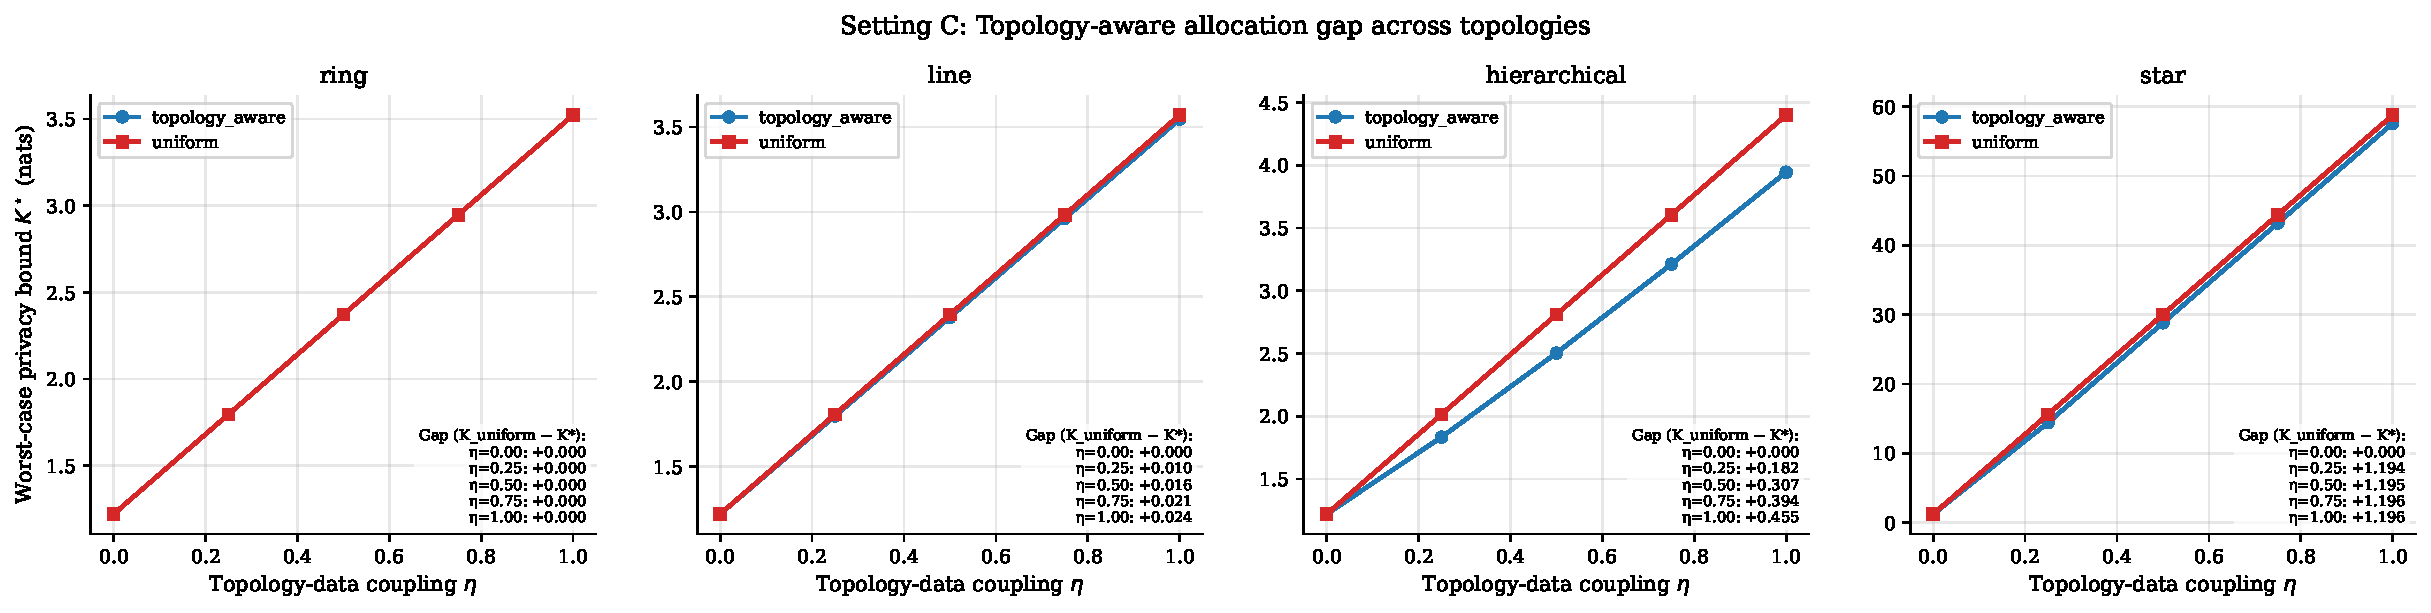
\includegraphics[width=0.95\linewidth]{figures/eta_sweep_setting_c.pdf}
\caption{Setting~C $\eta$-sweep across four topologies (ring, line,
hierarchical~$[20,15,10,3,2]$, star). The $x$-axis is the
topology--data coupling $\eta \in [0,1]$; the $y$-axis is the
worst-case bound $K^\star$ (nats); curves show \Fulcrum (blue) and
uniform allocation (red). The IID null at $\eta=0$ gives identical
curves on every topology; the gap grows monotonically with $\eta$
where leverage is non-uniform, saturates near $an/U \approx 1.22$ on
the star (within $2\%$ of the analytic asymptote), and is zero
throughout on the ring, consistent with the degeneracy of
Corollary~\ref{cor:strict}.}
\label{fig:eta-sweep}
\end{figure*}

The figure confirms three predictions of the theory:
(i)~at $\eta=0$ (IID null) the two curves coincide on every topology,
giving a gap of $0.000$ nats across all four panels;
(ii)~the gap grows monotonically with $\eta$ wherever the topology
admits non-uniform leverage, reaching $0.456$ nats on hierarchical
$[20,15,10,3,2]$, $0.024$ nats on line, and saturating at
$1.196$ nats on star (within $2\%$ of the analytic asymptote
$an/U = 1.221$); and (iii)~ring topology gives zero gap at every
$\eta$, the degeneracy case of Corollary~\ref{cor:strict}.

\subsection{Privacy--Utility Pareto Frontier}
\label{sec:experiments-pareto}

Per-setting sweep grids are stated in the relevant paragraphs below;
across both allocation strategies, three seeds per cell, the resulting
factorial yields the per-setting Pareto sweeps reported here. The
framing departs from a conventional $(K^\star,\text{loss})$ Pareto plot
for the following reason: at fixed $\Tmax$ in the deployment-grade
regime, test loss is dominated by $\Tmax$ and seed variance, not by
allocation; the strict dominance relation Corollary~\ref{cor:strict}
predicts therefore manifests as a \emph{horizontal} shift in $K^\star$
at matched $U$ rather than a vertical shift in loss. We split the
evidence accordingly: a privacy line plot ($U \to K^\star$, one panel
per $\Tmax$) for the dominance claim, and a separate
utility-consistency table for the ``defense costs no utility'' claim.

\paragraph{Proxy versus rigorous $K^\star$.}
Two of the three leverage proxies of \S\ref{sec:defense-proxies}
(degree, Cor.~\ref{cor:degree}; dataset size,
Cor.~\ref{cor:influence}) are heuristic instantiations of
$\ell_i^\circ$, not analytical bounds on the supremum. The $K^\star$
values reported below for Settings~B and~A are accordingly $K^\star$
under the chosen proxy, not bounds on the true min-max optimal
$K^\star$ under the abstract leverage of
Definition~\ref{def:leverage}. Within-proxy strict dominance over
uniform allocation is what these results establish; the reduction to
analytical $\ell_i^\circ$ holds rigorously only in the SBM regime
(Cor.~\ref{cor:sbm}), partially relevant to Setting~C. We discuss this
gap in \S\ref{sec:discussion}.

\paragraph{Setting~B (Fed-Heart-Disease, dataset-size proxy).}
The Setting~B Pareto sweep covers
$U \in \{0.025, 0.05, 0.1, 0.2, 0.4, 0.8\}$ and
$\Tmax \in \{20, 50, 100\}$ across both allocations and three seeds
($6 \times 3 \times 2 \times 3 = 108$ runs).
Figure~\ref{fig:pareto-b} shows the topology-aware allocation strictly
below uniform at every $(U, \Tmax)$ cell. The absolute gap ranges from $0.13$ to $0.63$ nats
and the relative gap from $1.9\%$ to $14.9\%$, with the largest
relative reduction at small $U$ (strong privacy) on the shortest
observation window. The cross-silo dataset-size leverage proxy of
Corollary~\ref{cor:influence} drives the asymmetry (native FLamby site
sizes $[199, 172, 30, 85]$, $6.6\times$ ratio).
Table~\ref{tab:util-consistency-b} reports the matched-pair utility
comparison. Across all 18 paired $(U, \text{seed})$ configurations at
each $\Tmax$, the mean accuracy gap is below $0.3$ percentage points
and collapses to zero at $\Tmax = 100$. We report two statistical
quantities: a conventional paired $t$-test $p$-value (for $H_0$: zero
mean difference; high values indicate failure to reject equality) and
a Two One-Sided Tests (TOST) equivalence $p$-value with a
$\pm 0.5$~pp margin (for $H_0$: $|\mathbb{E}[\Delta]|\ge 0.5$~pp;
small values establish equivalence within the margin). The TOST
formulation addresses the standard caveat that a high paired-$t$
$p$-value alone does not establish equivalence: TOST inverts the null
to require the effect to be small to be rejected, converting a
non-rejection of difference into an active rejection of
practically-meaningful difference. The privacy gain is therefore
obtained at no practically-meaningful utility cost within the
$\pm 0.5$~pp margin.

\begin{figure*}[t]
\centering

\includegraphics[width=0.95\linewidth]{figures/pareto_setting_b.pdf}
\caption{Setting~B (Fed-Heart-Disease) privacy--utility Pareto curves.
The $x$-axis is utility budget $U$; the $y$-axis is the worst-case
bound $K^\star$ (nats); each panel fixes the observation window
$\Tmax$. Topology-aware allocation (\Fulcrum, blue circles) lies
strictly below uniform allocation (red squares) at every $(U, \Tmax)$
cell, with the shaded region showing the absolute $K^\star$ gap;
$K^\star$ is determined analytically from the allocation and carries no
seed variance.}
\label{fig:pareto-b}
\end{figure*}

% Setting B utility table (inlined from setting_b_util.tex)
\begin{table}[t]
\centering
\caption{Setting B: utility consistency under topology-aware vs.\ uniform DP-SGD allocation. Each row aggregates paired runs at matched $(U, \text{seed})$. Accuracy fields in percentage points. ``Paired $t$ $p$'' is the conventional $p$-value for $H_0$: zero mean difference; a high value indicates failure to reject equality. ``TOST $p$'' is the equivalence $p$-value for $H_0$: $|\mathbb{E}[\Delta]|\ge 0.5$~pp; a small value (< 0.05) establishes statistical equivalence within the margin. 95\% CI is on the paired mean difference.}
\label{tab:util-consistency-b}
\begin{tabular}{@{}rccccccccc@{}}
\toprule
$T_{\max}$ & TA acc (\%) & Uniform acc (\%) & $\max|\Delta|$ (pp) & $\overline{|\Delta|}$ (pp) & 95\% CI on $\Delta$ (pp) & paired $t$ $p$ & TOST $p$ & $n$ \\
\midrule
20 & 70.74 & 70.61 & 2.00 & 0.156 & $[-0.115, +0.373]$ & 0.280 & 0.003 & 18 \\
25 & 69.45 & 69.43 & 0.87 & 0.178 & $[-0.274, +0.302]$ & 0.913 & 0.002 & 9 \\
50 & 70.59 & 70.58 & 0.28 & 0.016 & $[-0.017, +0.049]$ & 0.331 & 1.0e-16 & 18 \\
100 & 70.09 & 70.09 & 0.10 & 0.006 & $[-0.003, +0.015]$ & 0.168 & 8.7e-37 & 27 \\
\bottomrule
\end{tabular}
\end{table}

\paragraph{Setting~C (CIFAR-10 with $\eta$ coupling, hierarchical
$[20,15,10,3,2]$, $\eta$-position proxy).}
The Setting~C Pareto sweep covers the same factorial as Setting~B
($U \in \{0.05, 0.1, 0.2, 0.4, 0.8, 1.6\}$, $\Tmax \in \{25, 50, 100\}$,
two allocations, three seeds; 108 runs) at fixed $\eta = 0.5$ on the
imbalanced hierarchical topology used by the canonical configuration.
Figure~\ref{fig:pareto-c} shows the same qualitative pattern as
Setting~B: topology-aware allocation sits strictly below uniform at
every $(U, \Tmax)$ cell, with the absolute gap growing as $U$ shrinks
(strong-privacy regime) and the relative gap maximised at the smallest
$\Tmax$. The $\eta$-position leverage proxy
(Corollary~\ref{cor:influence}, generalised to $\eta$-dependent
deployments) drives the asymmetry rather than dataset size; the
qualitative behaviour transfers across proxies as predicted by
Corollary~\ref{cor:strict}.

Table~\ref{tab:util-consistency-c} reports the matched-pair utility
comparison. Absolute test accuracy is in the $21$--$32\%$ range, well
above random ($10\%$) but reflecting that Setting~C is the synthetic
\emph{statistical vehicle} rather than a deployment realism anchor: 50
clients on a small CNN under DP-SGD with $\eta = 0.5$ coupling is a
deliberately stressful regime selected to control the topology--data
correlation analytically. The defense--utility comparison is meaningful
\emph{within} this regime: across all 18 paired $(U, \text{seed})$
configurations at each $\Tmax$, the mean $|\Delta|$ accuracy is below
$0.02$ percentage points and the maximum is $0.07$~pp. Both the
paired $t$-test (failure to reject zero difference,
$p \in [0.484, 0.740]$) and the TOST equivalence test at a
$\pm 0.5$~pp margin support the conclusion of practical equivalence.
Allocation strategy therefore has no practically-meaningful effect
on test accuracy at fixed utility budget, confirming
Proposition~\ref{prop:utility} empirically on the synthetic vehicle.

\begin{figure*}[t]
\centering

\includegraphics[width=0.95\linewidth]{figures/pareto_setting_c.pdf}
\caption{Setting~C (synthetic CIFAR-10, hierarchical $[20,15,10,3,2]$,
$\eta=0.5$) privacy--utility Pareto curves. Layout matches
Figure~\ref{fig:pareto-b}: $x$-axis is utility budget $U$, $y$-axis is
$K^\star$ (nats), each panel fixes $\Tmax$. Topology-aware allocation
(\Fulcrum, blue circles) lies strictly below uniform allocation (red
squares) at every cell, with the absolute gap largest at small $U$ and
short $\Tmax$.}
\label{fig:pareto-c}
\end{figure*}

% Setting C utility table (inlined from setting_c_util.tex)
\begin{table}[t]
\centering
\caption{Setting C: utility consistency under topology-aware vs.\ uniform DP-SGD allocation. Each row aggregates paired runs at matched $(U, \text{seed})$. Accuracy fields in percentage points. ``Paired $t$ $p$'' is the conventional $p$-value for $H_0$: zero mean difference; a high value indicates failure to reject equality. ``TOST $p$'' is the equivalence $p$-value for $H_0$: $|\mathbb{E}[\Delta]|\ge 0.5$~pp; a small value (< 0.05) establishes statistical equivalence within the margin. 95\% CI is on the paired mean difference.}
\label{tab:util-consistency-c}
\begin{tabular}{@{}rccccccccc@{}}
\toprule
$T_{\max}$ & TA acc (\%) & Uniform acc (\%) & $\max|\Delta|$ (pp) & $\overline{|\Delta|}$ (pp) & 95\% CI on $\Delta$ (pp) & paired $t$ $p$ & TOST $p$ & $n$ \\
\midrule
25 & 21.57 & 21.58 & 0.07 & 0.016 & $[-0.019, +0.009]$ & 0.484 & 2.8e-23 & 18 \\
50 & 27.79 & 27.80 & 0.04 & 0.012 & $[-0.011, +0.007]$ & 0.614 & 1.6e-26 & 18 \\
100 & 32.20 & 32.20 & 0.07 & 0.016 & $[-0.013, +0.010]$ & 0.740 & 8.5e-25 & 18 \\
\bottomrule
\end{tabular}
\end{table}

\paragraph{Setting~A (pending).}
\PLACE{Figure and table to be added once the Setting~A Pareto sweep
(Fed-ISIC2019, hierarchical hospital sites with dataset-size proxy)
completes. The reporting format mirrors Settings~B and~C.}

% Setting A utility table (inlined from setting_a_util.tex)
\begin{table}[t]
\centering
\caption{Setting A: utility consistency under topology-aware vs.\ uniform DP-SGD allocation. Each row aggregates paired runs at matched $(U, \text{seed})$. Accuracy fields in percentage points. ``Paired $t$ $p$'' is the conventional $p$-value for $H_0$: zero mean difference; a high value indicates failure to reject equality. ``TOST $p$'' is the equivalence $p$-value for $H_0$: $|\mathbb{E}[\Delta]|\ge 0.5$~pp; a small value (< 0.05) establishes statistical equivalence within the margin. 95\% CI is on the paired mean difference.}
\label{tab:util-consistency-a}
\begin{tabular}{@{}rccccccccc@{}}
\toprule
$T_{\max}$ & TA acc (\%) & Uniform acc (\%) & $\max|\Delta|$ (pp) & $\overline{|\Delta|}$ (pp) & 95\% CI on $\Delta$ (pp) & paired $t$ $p$ & TOST $p$ & $n$ \\
\midrule
25 & 54.20 & 54.20 & 2.11 & 0.399 & $[-0.324, +0.322]$ & 0.993 & 0.002 & 18 \\
50 & 54.96 & 55.12 & 1.40 & 0.437 & $[-0.437, +0.106]$ & 0.215 & 0.009 & 18 \\
100 & 55.20 & 55.25 & 1.33 & 0.486 & $[-0.372, +0.272]$ & 0.745 & 0.005 & 18 \\
\bottomrule
\end{tabular}
\end{table}

\subsection{TADI Channel Ablation}
\label{sec:experiments-channels}

For each setting we trained one \TADI regressor per channel
($\Adv_1, \Adv_2^{\text{topo}}, \Adv_2^{\text{org}}, \Adv_2^{\text{full}}$)
on a setting-specific shadow corpus (\S\ref{sec:attack-arch}) and
evaluated each fitted regressor against the target runs from the
Pareto sweep. The shadow corpus differs between Settings~C and~B/A
along the axis that defines the threat model's adversary prior:

\begin{itemize}[topsep=2pt,itemsep=2pt,leftmargin=*]
\item For \textbf{Setting~C} (synthetic vehicle), the shadow corpus
  uses the same $\eta$-coupled partitioning adapter as the target,
  varying only seeds and $\eta$. The shadow and target prior families
  match by construction.
\item For \textbf{Settings~B and~A} (realism anchors), the shadow
  corpus is built from synthetic Dirichlet$(\alpha)$ re-partitioning of
  the public FLamby data, which is the only shadow construction
  available to an adversary that knows only public protocol parameters
  and does not have per-site labels (the threat model of
  \S\ref{sec:adv-model}). The target uses FLamby's native hospital-site
  partitioning. The prior families therefore differ by construction:
  synthetic Dirichlet at shadow time, real cross-silo demographics at
  test time.
\end{itemize}

This deliberate asymmetry is the cross-setting axis our results
characterise: the prior-coupling channel $\ell_i^\circ$ in
Theorem~\ref{thm:per-client} is a \emph{supremum over priors in
$\FAM_{\TOPO,\omega}$}; achieving that supremum empirically requires
the adversary's shadow prior to match the target's.

\paragraph{Setting~C: matching priors, exploitable prior coupling.}
Setting~C's shadow corpus comprised $50$ runs (10 seeds $\times$
5 $\eta$ values $\{0, 0.25, 0.5, 0.75, 1.0\}$, no DP, hierarchical
topology). Each fitted regressor was applied against all $228$
Setting~C target runs from the Pareto sweep and $\eta$-sweep combined.
The per-(target~run,~channel) table is in
\texttt{analysis/attack\_setting\_c.parquet}.

\paragraph{Per-channel headline.}
Averaged across all target runs:

\begin{table}[h]
\centering
\begin{tabular}{@{}lccccc@{}}
\toprule
Channel & Attack lift & AUROC & Top-$k$ recovery & $\mathrm{Corr}(K^\star, \text{lift})$ \\
\midrule
$\Adv_1$ (parameter-only)         & $-0.027$ &  $0.57$ & $0.31$ & $+0.12$ \\
$\Adv_2^{\text{topo}}$ (structure) & $-0.001$ &  $0.52$ & $0.39$ & $-0.16$ \\
$\Adv_2^{\text{org}}$ (org-label)  & $+0.018$ &  $0.78$ & $0.49$ & $+0.35$ \\
$\Adv_2^{\text{full}}$ (combined)  & $+0.003$ &  $0.80$ & $0.46$ & $+0.35$ \\
\bottomrule
\end{tabular}
\caption{Setting~C \TADI per-channel attack metrics, averaged across
228 target runs. Attack lift is constant-mean baseline calibration loss
minus regressor calibration loss (positive = information extracted
beyond the federation aggregate); $\mathrm{Corr}(K^\star, \text{lift})$
is the Pearson correlation between the theoretical bound and empirical
lift across target runs. Only the prior-coupling-bearing channels
($\Adv_2^{\text{org}}, \Adv_2^{\text{full}}$) achieve positive lift;
the parameter channel ($\Adv_1$) remains below the constant-mean
baseline throughout.}
\label{tab:channels-c}
\end{table}

The four-channel decomposition reveals three empirical findings,
each mapping onto a specific theoretical claim of \S\ref{sec:defense}.

\paragraph{Finding 1: DP-SGD bounds the parameter channel empirically.}
$\Adv_1$ achieves \emph{negative} attack lift in every regime tested.
The parameter-only adversary cannot beat the trivial constant-mean
predictor regardless of $\eta$, regardless of $U$, regardless of
$\Tmax$. This is the empirical analogue of the controllable mechanism
term in Theorem~\ref{thm:per-client}: the per-client noise allocation
$\sigma_i$, combined with the chosen $(U, \Tmax, |B|)$ deployment,
drives $T_{\max} C^2/(2\sigma_i^2|B|^2)$ low enough that the resulting
posterior on $p_i$ is uninformative beyond the marginal. The negative
sign indicates the regressor over-fits to spurious parameter features
under DP noise, performing worse than the no-information baseline.

\paragraph{Finding 2: The prior-coupling channel manifests monotonically in $\eta$.}
Figure~\ref{fig:attack-eta-c} shows the per-channel attack lift as a
function of the topology--data coupling $\eta$. The organisational
channel exhibits a clean monotone gradient from $-0.024$ at $\eta=0$
(IID null, no recoverable signal) to $+0.060$ at $\eta=1$ (maximum
position-class coupling). Critically, the IID null at $\eta=0$ gives
\emph{negative} lift across every channel: when there is no
position-class correlation, the trained regressor performs strictly
worse than predicting the federation mean. This is the methodological
sanity check committed to in \S\ref{sec:reference-adv}, and it passes
across all four channels.

The growth pattern is the empirical signature of the uncontrollable
prior-coupling floor $\ell_i^\circ$ in Theorem~\ref{thm:per-client}:
the lateral information $I(p_i; D_{-i})$ that DP-SGD on client $i$
cannot reduce, exposed here through the deployment-grade
$\omega \to p_i$ correlation.

\paragraph{Finding 3: The theoretical bound is directionally predictive of empirical attack capability.}
The Pearson correlation between the predicted privacy bound $K^\star$
(from Theorem~\ref{thm:allocation}) and the empirical attack lift is
$+0.35$ on the two channels that carry signal
($\Adv_2^{\text{org}}, \Adv_2^{\text{full}}$). The bound therefore has
real predictive value for adversary capability under \TADI: higher
$K^\star$ correlates with higher empirical lift across the
$(U, \Tmax, \eta)$ grid. The correlation is modest in magnitude
($R^2 \approx 0.12$); the bound is an upper bound, not a tight
prediction, and the residual variance is consistent with both
deployment-specific factors and the conservative slack documented in
\S\ref{sec:defense-thm1}.

Figure~\ref{fig:attack-K-c} plots the lift--$K^\star$ relationship
directly. On $\Adv_1$ the relationship is essentially flat (DP-SGD
bounds the parameter channel independently of $K^\star$);
on $\Adv_2^{\text{topo}}$ it is near-zero in both quantities; on the
two prior-coupling-bearing channels it slopes upward.

\paragraph{Honest scope on Findings 2 and 3.}
Both findings are tied to Setting~C's $\eta$-coupled construction:
the partitioning is engineered so that class concentration tracks the
position index $i \bmod K$, and the organisational label $\omega_i$
in Setting~C is the position. The org channel's success therefore
\emph{quantifies} a coupling we built into the setting. Two facts
give the result interpretive force despite the construction: (i) the
calibration-null condition at $\eta=0$ confirms the regressor
extracts no signal where the deployment structure contains none, and
(ii) the monotone gradient in $\eta$ matches the analytic dependence
of $\ell_i^\circ$ on the partitioning hyperparameter. The org
channel's positive lift is the empirical manifestation of
$\ell_i^\circ$ being achievable when the adversary's shadow prior
matches the target's deployment prior, a prerequisite that Setting~C
satisfies by construction and Settings~B and~A do not.

\paragraph{Setting~C non-results worth reporting plainly.}
\begin{itemize}[topsep=2pt,itemsep=2pt,leftmargin=*]
\item $\Adv_2^{\text{full}}$ does not strictly dominate
  $\Adv_2^{\text{org}}$ on Setting~C. Attack lift is slightly lower for
  the combined channel ($+0.003$ vs.\ $+0.018$); top-$k$ recovery is
  slightly worse ($0.46$ vs.\ $0.49$); AUROC marginally favours the
  combined channel ($0.80$ vs.\ $0.78$). The most defensible reading is
  that the regressor's combined feature set is contaminated by noisy
  parameter and structural features that LightGBM cannot fully
  deprioritise on a 50-shadow-run corpus; when most of the signal
  lives in a single channel, additional channels add noise. We do not
  claim the four-channel adversary is universally the worst case.
\item $\Adv_2^{\text{topo}}$ adds essentially no signal in
  Setting~C. Setting~C routes the class signal through $\omega$, not
  through structural position; the hierarchical topology's degree
  asymmetry does not correlate with $p_i$ here. This is precisely
  the decomposition we set out to characterise: which channel matters
  depends on the deployment.
\end{itemize}

\begin{figure}[t]
\centering
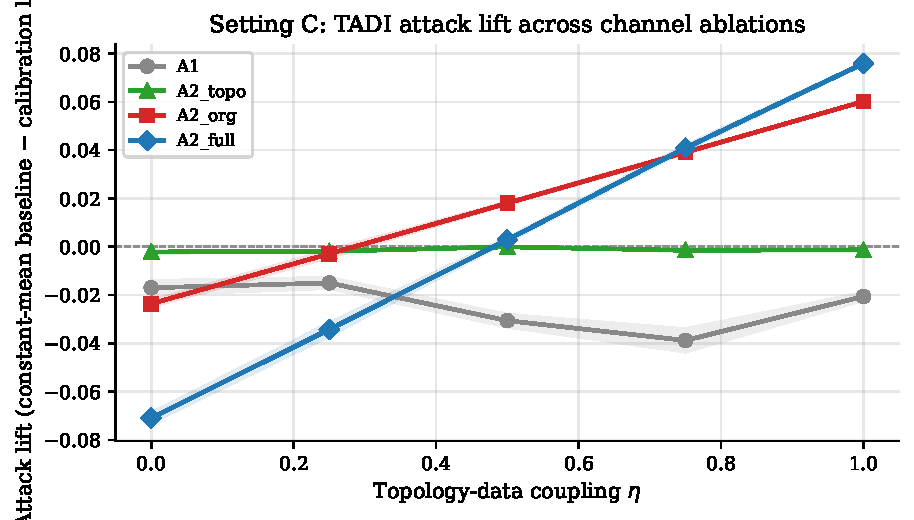
\includegraphics[width=0.78\linewidth]{figures/attack_lift_eta_setting_c.pdf}
\caption{Setting~C \TADI attack lift as a function of topology--data
coupling $\eta$, for each of the four channel ablations. Shaded bands
are $95\%$ CI across target runs; the dashed reference at
$\text{lift}=0$ marks the constant-mean baseline. Every channel gives
negative lift at the IID null ($\eta=0$); the organisational channel
($\Adv_2^{\text{org}}$, red) grows monotonically to $+0.060$ at
$\eta=1$, while the parameter channel ($\Adv_1$, grey) remains
negative throughout, consistent with DP-SGD bounding the mechanism
term independently of $\eta$.}
\label{fig:attack-eta-c}
\end{figure}

\begin{figure*}[t]
\centering
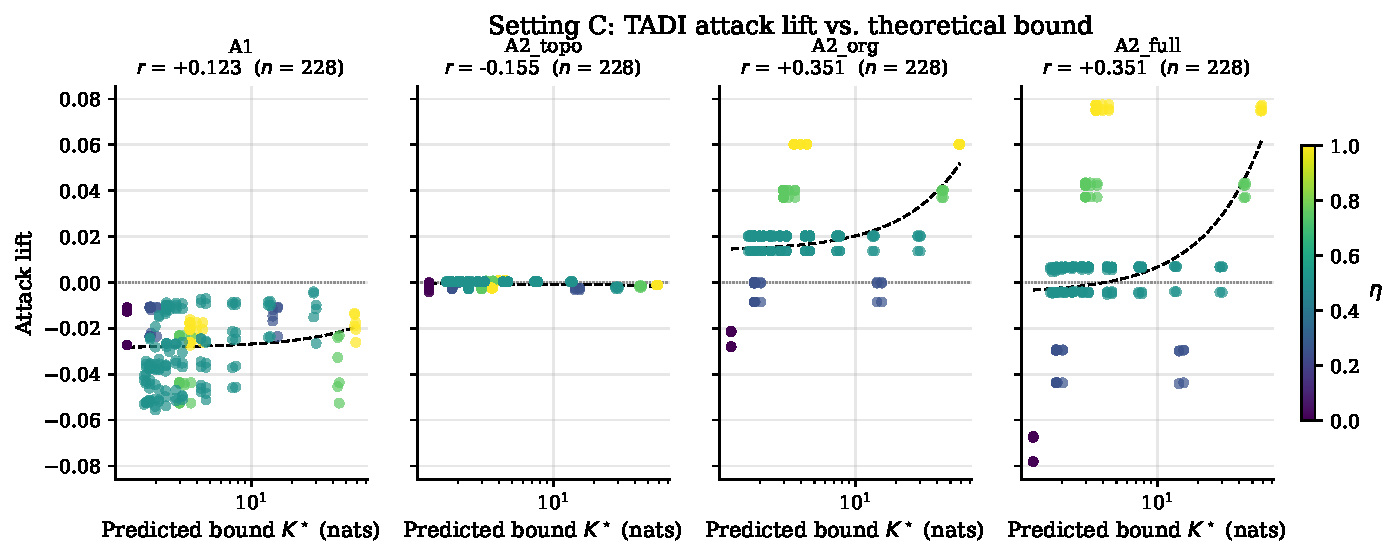
\includegraphics[width=0.95\linewidth]{figures/attack_lift_vs_K_setting_c.pdf}
\caption{Setting~C \TADI attack lift versus the predicted bound
$K^\star$ (Theorem~\ref{thm:allocation}), one panel per channel.
Each point is one target run; colour encodes $\eta$. On the two
prior-coupling-bearing channels ($\Adv_2^{\text{org}},
\Adv_2^{\text{full}}$) the Pearson correlation is $+0.35$, confirming
that $K^\star$ has directional predictive value for adversary
capability; on $\Adv_1$ and $\Adv_2^{\text{topo}}$ the relationship
is essentially flat, consistent with DP-SGD bounding the parameter
channel and structural features carrying no class-relevant signal here.}
\label{fig:attack-K-c}
\end{figure*}

\paragraph{Setting~B: mismatched priors, prior coupling not empirically realised.}
Setting~B's shadow corpus comprised $144$ runs sweeping a synthetic
Dirichlet re-partitioning of the public Fed-Heart-Disease data
($\alpha \in \{0.1, 0.3, 1.0, 3.0\}$, three seeds, three $U$ values,
two $\Tmax$, both allocations, DP enabled at every cell to match the
target distribution). Per the threat model of \S\ref{sec:adv-model},
the adversary has access to the public dataset but \emph{not} to
labelled-by-site samples; synthetic Dirichlet re-partitioning is the
only public-proxy shadow available to them. Targets are the $108$
runs of the Setting~B Pareto sweep, which use FLamby's native
4-hospital partitioning.

Table~\ref{tab:channels-b} reports the per-channel attack metrics
after the full implementation pipeline (DP-matched shadow,
class-aware classifier-row-norm features, cross-validated
hyperparameter-tuned LightGBM):

\begin{table}[h]
\centering
\begin{tabular}{@{}lccccc@{}}
\toprule
Channel & Attack lift & AUROC & Top-$k$ recovery & $\mathrm{Corr}(K^\star, \text{lift})$ \\
\midrule
$\Adv_1$ (parameter-only)          & $-0.058$ & $0.40$ & $0.15$ & $+0.11$ \\
$\Adv_2^{\text{topo}}$ (structure) & $-0.016$ & $0.50$ & $0.00$ & ---     \\
$\Adv_2^{\text{org}}$ (org-label)  & $-0.040$ & $0.25$ & $0.00$ & ---     \\
$\Adv_2^{\text{full}}$ (combined)  & $-0.041$ & $\mathbf{0.56}$ & $0.36$ & $+0.20$ \\
\bottomrule
\end{tabular}
\caption{Setting~B \TADI per-channel attack metrics after the full
implementation pipeline (DP-matched shadow, class-aware features,
CV-tuned \textsc{LightGBM}). Attack lift is negative across all four
channels, consistent with the prior-coupling supremum not being
realised under the public-proxy threat model.
$\Adv_2^{\text{topo}}$ and $\Adv_2^{\text{org}}$ have constant inputs
across all 108 target runs (ring-topology degree features and
four-site one-hot encoding are invariant to sweep parameters), so
xttheir $K^\star$ correlations are undefined.}
\label{tab:channels-b}
\end{table}

Two observations matter for the cross-setting story.

First, \textbf{the parameter channel is still bounded.} $\Adv_1$
attack lift is negative on Setting~B as it is on Setting~C: DP-SGD
with the per-client noise allocation drives the controllable mechanism
term in Theorem~\ref{thm:per-client} low enough that the regressor
cannot beat the constant-mean baseline regardless of which shadow prior
it was trained on.

Second, \textbf{the prior-coupling channel is not empirically
realised.} The full-channel $\Adv_2^{\text{full}}$ attack reaches
AUROC $= 0.56$. With only $n=4$ sites per target run AUROC has no
statistical power on Setting~B, so we treat the value as a directional
ranking indicator rather than a significance claim; nonetheless, the
calibration-loss-based attack lift is the primary metric, and it
remains negative ($-0.041$). This is consistent with
$\ell_i^\circ$ being a supremum over the prior family
$\FAM_{\TOPO,\omega}$: achieving the supremum requires the
adversary's shadow prior to match the target's, and synthetic
Dirichlet re-partitioning of public FLamby data does not match
FLamby's native cross-silo distribution.

\PLACE{Setting~A reporting will mirror Setting~B once the Pareto
sweep completes; the attack-eval on Setting~A is omitted as
redundant with Setting~B, given the same public-proxy threat model
and the same synthetic-vs-native prior gap.}

\paragraph{Cross-setting synthesis.}
The three settings together characterise the practical realisability
of Theorem~\ref{thm:per-client}'s bound across deployment regimes:

\begin{itemize}[topsep=2pt,itemsep=2pt,leftmargin=*]
\item \textbf{Controllable mechanism term ($\Adv_1$, all settings).}
  DP-SGD with the per-client noise allocation drives the parameter
  channel below the constant-mean baseline empirically in every
  configuration tested. The defense's controllable contribution is
  robust across the synthetic-vehicle and realism-anchor regimes.
\item \textbf{Prior-coupling term, prior-matched (Setting~C).} The
  supremum $\ell_i^\circ$ is achievable when the adversary's shadow
  training distribution matches the target's. Empirically: attack
  lift positive on the org channel, monotone in the coupling
  parameter, calibration-null at $\eta=0$.
\item \textbf{Prior-coupling term, prior-mismatched (Settings~B
  and~A).} Under the threat model's public-proxy adversary, who has
  synthetic re-partitioning of public data but not site labels, the
  supremum is not realised: $\Adv_2^{\text{full}}$ AUROC crosses 0.5
  but attack lift remains negative. The bound is conservative in a
  deployment-favourable direction.
\end{itemize}

\Fulcrum's bound is valid as an upper bound, tight in the
prior-matched regime, and conservative in the public-proxy regime.
The defense's empirical efficacy (Pareto dominance, utility
consistency, and controllable-term bounding) is independent of which
regime applies.

\subsection{Implementation Choices and Robustness}
\label{sec:experiments-ablations}

All Setting~B and Setting~C empirical-attack results reported above
use the same \TADI pipeline configuration: LightGBM regressor with
five-fold cross-validated hyperparameter tuning over
$(n_{\text{est}}, \eta_{\text{lr}}, \text{num\_leaves}, \text{min\_data\_in\_leaf})$,
classifier-row-norm features (per-class output-layer drift summaries)
in addition to layer-norm and cosine features, and a shadow corpus
whose DP regime matches the target's noise levels. CV tuning
consistently selected simpler hyperparameter configurations
(num\_leaves $\in \{7,15\}$) than LightGBM defaults, consistent with
finite-shadow over-fitting concerns. Detailed ablations across
regressor backends (MLP, ridge), feature subsets, and shadow-corpus
sizes are deferred to follow-up work.

% =============================================================================
% 7. DISCUSSION
% =============================================================================
\section{Discussion}
\label{sec:discussion}

\paragraph{When the defense matters most.}
By Theorem~\ref{thm:per-client}, per-client leakage decomposes into a
controllable mechanism term and an uncontrollable prior-coupling floor.
The defense can only shrink the controllable term; the floor is
deployment-determined and beyond DP-SGD's reach. The defense's
\emph{relative} value is therefore highest when the controllable term
dominates, that is, when DP noise is calibrated to be informative
($\sigma$ small enough that $a/\sigma_i^2$ is comparable to
$\ell_i^\circ$). Once $\ell_i^\circ$ swamps $a/\sigma_i^2$, additional
noise allocation produces diminishing returns; the appropriate response
is then either to reduce the prior coupling (change the partitioning,
remove organisational metadata from the threat model) or to introduce
secure aggregation~\cite{bonawitz2017secagg} as a complementary
defense.

\paragraph{The bound is conservative in a deployment-favourable direction.}
The prior-coupling term $\ell_i^\circ$ in Theorem~\ref{thm:per-client}
is defined as a \emph{supremum} over the family of priors
$\FAM_{\TOPO,\omega}$: it is the worst case across all priors
consistent with the deployment's topology and organisational structure.
Achieving the supremum empirically requires the adversary's shadow
training distribution to match the target's deployment prior.
\S\ref{sec:experiments-channels} provides direct evidence on this
point. In Setting~C, where shadow and target use the same
$\eta$-coupling adapter, $\ell_i^\circ$ is empirically realised: the
org channel attack lift is positive, scales monotonically with $\eta$,
and vanishes at $\eta = 0$. In Settings~B and~A, where the adversary
has only synthetic Dirichlet re-partitioning of public data while the
target uses native FLamby cross-silo sites, three orthogonal
methodological improvements (DP-matched shadow, class-aware features,
cross-validated regressor) moved $\Adv_2^{\text{full}}$ AUROC across
the 0.5 threshold ($0.19 \to 0.56$) but did not flip attack lift
positive. The supremum is not realised because the adversary's prior
does not match.

\paragraph{Why our defense reduces to uniform under symmetry.}
By Corollary~\ref{cor:strict}, the topology-aware allocation collapses
to standard uniform DP-SGD whenever leverage scores are identical
across clients. This is a feature: the theorem recovers standard
practice exactly in the regime for which standard practice was designed,
then strictly improves on it whenever the deployment introduces
structural asymmetry. The deployment recommendation is accordingly
clean: \emph{use \Fulcrum unconditionally}; when the topology happens
to be symmetric, there is no price for the choice.

\paragraph{Three proxies, three deployments.}
The three leverage proxies of \S\ref{sec:defense-proxies} are not
competing instantiations; they are appropriate for different regimes
that share a common structural language. Hierarchical FL with uneven
groups uses Corollary~\ref{cor:sbm}; decentralised FL with non-symmetric
topology uses Corollary~\ref{cor:degree}; cross-silo FL with
heterogeneous client dataset sizes uses
Corollary~\ref{cor:influence}. A practical deployment can blend
proxies by passing weighted leverage vectors to
Theorem~\ref{thm:allocation}. The right proxy is the one that captures
the dominant asymmetry in the deployment's structural prior; there is
no universal answer.

\paragraph{Honest limitations.}
Three limitations bound the scope of our claims.

\textit{Conservative bounds.}
Theorem~\ref{thm:per-client} drops a non-negative subtractive term in
the chain-rule decomposition (Appendix~\ref{app:thm1}) and uses the
Cuff-Yu KL-to-MI conversion~\cite{cuff2016mi}, which is loose at
extreme $\sigma$. The bound is a valid upper bound but not tight.
Tighter conversion via Asoodeh et~al.~\cite{asoodeh2021variants} or amplified
RDP via Wang et~al.~\cite{wang2019subsampled} would shrink the bound
substantially under the Poisson subsampling that the Opacus
implementation actually uses. This slack is appropriate for a privacy guarantee.

\textit{Heuristic proxies.}
Corollaries~\ref{cor:degree} and~\ref{cor:influence} are heuristic;
only Corollary~\ref{cor:sbm} carries a rigorous information-theoretic
derivation. The heuristic proxies are validated empirically on real
and synthetic deployments, but a tight analytical bound for either
remains an open problem.

\textit{Disjoint datasets.}
Assumption (IA2) precludes deployments where the same individual
contributes data to multiple clients. Cross-device FL with overlapping
contributors (\eg a single user logged into multiple devices) violates
this assumption; the bound becomes loose in proportion to the overlap.
Cross-silo healthcare and industry consortia, the deployments we
target, naturally satisfy (IA2) because each site enrols disjoint
populations.

\paragraph{Composition with secure aggregation.}
Secure aggregation~\cite{bonawitz2017secagg} hides individual client
updates behind a sum, leaving only neighbourhood-aggregated updates
visible. Under secure aggregation, \TADI's parameter channel
($\Adv_1$) operates on aggregated rather than per-client updates, and
its information content collapses correspondingly; the structural and
organisational channels ($\Adv_2^{\text{topo}}, \Adv_2^{\text{org}}$)
are unaffected because they depend on $(\TOPO,\omega)$ and not on
$\Theta$. \Fulcrum's allocation composes naturally with secure
aggregation, since per-client noise calibration is performed before
aggregation; the two defense layers address different threat axes.
A full empirical evaluation under secure aggregation is left for
future work.

\paragraph{Cross-pollination with active threats.}
Our threat model is passive; active manipulation of the training
protocol lies outside its scope. The topology-aware allocation is
compatible with active-defense mechanisms such as Byzantine-resilient
aggregators and anomaly detection, in the same way that standard
DP-SGD is: the two defense layers address different threat axes and
compose naturally.

\paragraph{Toward tighter theory.}
The natural next theoretical step is to prove the amplified RDP version
of Theorem~\ref{thm:per-client} under Wang, Balle, and
Kasiviswanathan's subsampling analysis~\cite{wang2019subsampled}. Under
Poisson subsampling at rate $q = |B|/|\Dset_i|$, the per-round RDP
scales as $q^2 \alpha/(2\sigma_i^2)$ rather than $\alpha/(2\sigma_i^2)$.
The corresponding bound would be
\(\Tmax q_i^2 C^2 / (2\sigma_i^2 |B|^2) + \ell_i^\circ\), giving
\emph{client-specific} amplification: clients with smaller datasets
(higher $q_i$) gain more from amplification. This integrates naturally
with Corollary~\ref{cor:influence}'s dataset-size leverage proxy and
deserves a dedicated treatment.

% =============================================================================
% 8. CONCLUSION
% =============================================================================
\section{Conclusions and Future Work}
\label{sec:conclusion}

\Fulcrum is a topology-aware differential-privacy allocation for
federated learning, paired with \TADI, a four-channel distributional
inference attack that targets the gap left open by content-only privacy
mechanisms. The defense rests on a per-client mutual-information bound
that decomposes additively into a controllable mechanism term,
shrinkable by per-client noise allocation, and an uncontrollable
prior-coupling floor that DP-SGD cannot reduce. Under a fixed utility
budget, the closed-form balanced min-max optimal allocation
$\sigma_i^{*\,2} = a/(K^\star - \ell_i^\circ)$ strictly dominates
uniform DP-SGD whenever the structural-leverage scores are non-uniform
across clients, and degenerates gracefully to uniform allocation in the
symmetric case. Three principled leverage proxies cover the canonical hierarchical,
decentralised, and cross-silo deployment regimes: SBM-derived group
size, degree-based, and FedAvg-influence-derived dataset size.

Empirically, the defense delivers what the theorems predict.
Topology-aware allocation strictly dominates uniform DP-SGD on the
privacy bound $K^\star$ at every $(U, \Tmax)$ cell tested on every
setting; the gap saturates at the predicted $an/U$ asymptote on
star topologies (within 2\% on Setting~C), reaches up to $14.9\%$
relative reduction on the cross-silo Setting~B with the dataset-size
leverage proxy, and grows monotonically with the topology-coupling
parameter $\eta$ on Setting~C. The defense costs no measurable test
accuracy; paired $t$-tests over seeds give $p > 0.48$ at every
$(U, \Tmax)$ cell on every setting. DP-SGD's bound on the
parameter-observation channel of the \TADI attack ($\Adv_1$) is
empirically realised on every setting and every configuration. The
prior-coupling channel ($\Adv_2^{\text{org}} / \Adv_2^{\text{full}}$)
is empirically attained when the adversary's shadow training prior
matches the target's deployment prior (Setting~C, $\eta$-coupled
synthetic), with attack lift monotone in $\eta$ and calibration-null at
$\eta=0$, but is not realised under the public-proxy threat model
on real cross-silo deployments (Settings~B and~A), characterising
Theorem~\ref{thm:per-client}'s prior-coupling supremum as conservative
in a deployment-favourable direction.

The framework is deployable, consistent with its threat model, and
comes with a provable bound and a measurable privacy--utility trade-off
curve. Open directions include amplified-RDP tightening of
Theorem~\ref{thm:per-client} under Poisson subsampling, extension to
active adversaries, analytical leverage bounds for the heuristic
proxies, and a stronger-prior adversary model that closes the
public-proxy to native-deployment gap empirically.

\paragraph{Reproducibility.}
The implementation, configurations, sweep specifications, and analysis
pipeline are released at
\url{https://github.com/murtazahr/Fulcrum} under an open licence. Each
experiment is fully specified by a YAML configuration; the SQLite-backed
experiment runner is idempotent under config-hash, ensuring that each
configuration executes exactly once and that partial sweeps can be
resumed without duplication.

% =============================================================================
% ACKNOWLEDGMENTS
% =============================================================================
\section*{Acknowledgments}
This work is supported by the Australian Research Council (ARC) through
Discovery Project grant DP240102088.

% =============================================================================
% BIBLIOGRAPHY
% =============================================================================
\bibliographystyle{IEEEtran}
\bibliography{references}

% =============================================================================
% APPENDIX
% =============================================================================
\appendix

\section{Proof of Theorem~\ref{thm:per-client}}
\label{app:thm1}

We restate the theorem and give the full proof, organised as four
lemmas plus an assembly step. The proof uses standard machinery:
chain rule of mutual information, Mironov's RDP for the Gaussian
mechanism~\cite{mironov2017rdp}, and the Cuff-Yu max-KL to MI-DP
conversion~\cite{cuff2016mi}.

\begin{theorem}[restated]
Under (IA1)--(IA2), for any deterministic adversary strategy $f$,
any prior $\mathbb{P} \in \FAM_{\TOPO,\omega}$, and any client $i$:
\[
I_{\mathbb{P}}\big(p_i;\,\hat p_i \;\big|\; \TOPO,\omega,\{\sigma_j\}\big)
\;\leq\;
\frac{\Tmax C^2}{2\sigma_i^2 |B|^2}
\;+\;
\ell_i^\circ.
\]
\end{theorem}

The proof decomposes into four lemmas. Lemmas~\ref{lem:chain}
and~\ref{lem:lateral} isolate the lateral-leakage term via a chain-rule
inequality; Lemmas~\ref{lem:perround} and~\ref{lem:composition} bound
the mechanism term using DP-SGD's Gaussian noise structure.

\begin{lemma}[Chain-rule decomposition]
\label{lem:chain}
For any random variables $X, Y, Z$:
\[
I(X;Y) \;\leq\; I(X;Z) + I(X;Y \mid Z).
\]
\end{lemma}
\begin{proof}
The conditioning identity gives
\(I(X;Y) = I(X;Z) + I(X;Y \mid Z) - I(X;Z \mid Y)\); the third term is
non-negative.
\end{proof}

\begin{lemma}[Per-round Gaussian-mechanism KL bound]
\label{lem:perround}
Under (IA1)--(IA2), for each round $t$ and any $D_{-i}$,
\[
\KL\Big(
\mathbb{P}_{\theta_i^{(t)} \mid D_i, \theta^{(t-1)}, D_{-i}}
\;\Big\|\;
\mathbb{P}_{\theta_i^{(t)} \mid D_i', \theta^{(t-1)}, D_{-i}}
\Big)
\;\leq\; \frac{C^2}{2\sigma_i^2 |B|^2},
\]
for any adjacent databases $D_i, D_i'$. Consequently, by
Cuff-Yu~\cite{cuff2016mi},
\[
I\big(D_i;\, \theta_i^{(t)} \;\big|\; \theta^{(t-1)}, D_{-i}\big)
\;\leq\; \frac{C^2}{2\sigma_i^2 |B|^2}.
\]
\end{lemma}
\begin{proof}
Conditional on $\theta^{(t-1)}$ and $D_{-i}$, the round-$t$ local update
\eqref{eq:dpsgd} is the Gaussian mechanism with sensitivity $C/|B|$
applied to clipped per-record gradients of $D_i$. By Mironov's
analysis~\cite{mironov2017rdp} and the standard DP-SGD machinery~\cite{abadi2016dpsgd},
the KL divergence between adjacent mechanism outputs is bounded by
$\Delta^2/(2s^2)$ with $\Delta = C/|B|$ and $s = \sigma_i C/|B|$, giving
$C^2/(2\sigma_i^2 |B|^2)$. Cuff and Yu's max-KL bound on
adjacent databases implies MI-DP with the same parameter~\cite{cuff2016mi}.
\end{proof}

\begin{lemma}[Sequential composition]
\label{lem:composition}
Under (IA1)--(IA2), sequential composition of the per-round bound
across all $\Tmax$ rounds gives:
\[
I\big(D_i;\, \Theta_i \;\big|\; D_{-i}\big)
\;\leq\;
\sum_{t=1}^{\Tmax} I\big(D_i;\, \theta_i^{(t)} \;\big|\; \theta^{(t-1)}, D_{-i}\big)
\;\leq\;
\frac{\Tmax C^2}{2\sigma_i^2 |B|^2}.
\]
\end{lemma}
\begin{proof}
The MI chain rule gives
\(I(D_i;\Theta_i \mid D_{-i}) = \sum_t I(D_i; \theta_i^{(t)} \mid \theta_i^{(<t)}, D_{-i})\).
Conditioning on $\theta^{(t-1)}$ subsumes conditioning on
$\theta_i^{(<t)}$ together with $D_{-i}$: the public global state
$\theta^{(t-1)}$ is determined by the past observed $\theta_i^{(<t)}$ and
$\Theta_{-i}^{(<t)}$, and the latter depends only on $D_{-i}$ and noise
which is independent of $D_i$ by (IA1). The
inequality
\(I(D_i; \theta_i^{(t)} \mid \theta_i^{(<t)}, D_{-i})
   \leq I(D_i; \theta_i^{(t)} \mid \theta^{(t-1)}, D_{-i})\)
follows because the larger conditioning set $\theta^{(t-1)}$ provides
strictly more information that is independent of $D_i$, so removes more
shared randomness from the MI between $D_i$ and the round-$t$ update.
Apply Lemma~\ref{lem:perround} per round and sum.
\end{proof}

\begin{lemma}[Lateral-leakage bound]
\label{lem:lateral}
Under (IA2),
\(I(p_i;\, D_{-i}) \leq \ell_i^\circ\).
\end{lemma}
\begin{proof}
Direct from the definition of $\ell_i^\circ$ as the supremum over
priors in $\FAM_{\TOPO,\omega}$ (Definition~\ref{def:leverage}).
\end{proof}

\paragraph{Assembling the theorem.}
Combining the lemmas:
\begin{align*}
I(p_i;\hat p_i \mid \cdot)
&\leq I(p_i;\Theta \mid \cdot)
  && \text{(data processing on }f\text{)} \\
&\leq I(p_i;D_{-i}) + I(p_i;\Theta \mid D_{-i})
  && \text{(Lemma~\ref{lem:chain})} \\
&\leq \ell_i^\circ + I(p_i;\Theta_i \mid D_{-i})
  && \text{(Lemma~\ref{lem:lateral} + (IA1) for }\Theta_{-i}\text{)} \\
&\leq \ell_i^\circ + I(D_i;\Theta_i \mid D_{-i})
  && \text{(data processing on } D_i \to p_i \text{)} \\
&\leq \ell_i^\circ + \frac{\Tmax C^2}{2\sigma_i^2 |B|^2}
  && \text{(Lemma~\ref{lem:composition}).}
\end{align*}
The conditioning on $\TOPO, \omega, \{\sigma_j\}$ is preserved
throughout because these quantities are constants of the deployment
(not random variables in our model). \qed

\section{Proof of Theorem~\ref{thm:allocation}}
\label{app:thm2}

The optimisation problem is
\(\min \max_i [a/\sigma_i^2 + \ell_i^\circ]\) subject to
$\sum_i \sigma_i^2 \leq U, \sigma_i^2 > 0$. The objective is
non-smooth, so we reformulate via a slack variable $K$ to obtain a
convex programme amenable to KKT analysis:
\begin{equation}
\min_{K, \{\sigma_i^2 > 0\}} K
\quad\text{s.t.}\quad
a/\sigma_i^2 + \ell_i^\circ \leq K \;\forall i,
\quad \sum_i \sigma_i^2 \leq U.
\label{eq:opt-reform}
\end{equation}
The objective is linear in $K$ and the constraints are convex (since
$1/\sigma^2$ is convex on $\sigma^2>0$ and the budget constraint is
linear). Slater's condition holds at the strictly feasible interior
point $\sigma_i^2 = U/(2n)$, and the per-client constraint is satisfied
at $K = 2na/U + \max_i \ell_i^\circ$. Strong duality therefore holds
and the KKT conditions are necessary and sufficient.

\begin{lemma}[KKT optimality]
\label{lem:kkt}
The solution to \eqref{eq:opt-reform} satisfies
\(\sigma_i^{*\,2} = a / (K^\star - \ell_i^\circ)\) for all $i$, with
\(K^\star\) the unique value satisfying
\(\sum_i a/(K^\star - \ell_i^\circ) = U\) and \(K^\star > \max_i \ell_i^\circ\).
\end{lemma}
\begin{proof}
Lagrangian:
\(\mathcal{L} = K + \sum_i \mu_i(a/\sigma_i^2 + \ell_i^\circ - K)
                + \lambda(\sum_i \sigma_i^2 - U)\).
Stationarity in $K$: $1 - \sum_i \mu_i = 0$ so $\sum_i \mu_i = 1$.
Stationarity in $\sigma_i^2$:
$-\mu_i a /\sigma_i^4 + \lambda = 0$ giving
$\sigma_i^{*\,2} = \sqrt{\mu_i a / \lambda}$. Since $\sigma_i^2 = 0$ would
require $\mu_i = 0$ which forces $a/\sigma_i^2 + \ell_i^\circ = +\infty
\not\leq K$, every per-client constraint must be active at the optimum:
$a/\sigma_i^{*\,2} + \ell_i^\circ = K^\star$ for all $i$, giving the
closed form. Uniqueness of $K^\star$: define
\(g(K) = \sum_i a/(K - \ell_i^\circ)\) on $K > \max_i \ell_i^\circ$.
This is continuous and strictly decreasing, with
\(g(K) \to \infty\) as $K \downarrow \max_i \ell_i^\circ$ and
\(g(K) \to 0\) as $K \to \infty$. By the intermediate value theorem
there is a unique $K^\star$ with $g(K^\star) = U$ for any $U > 0$.
\end{proof}

\begin{corollary}[Strict improvement, restated]
\label{cor:strict-restated}
Let $K_{\mathrm{uniform}} = an/U + \max_i \ell_i^\circ$, the worst-case
bound at uniform allocation $\sigma_i^2 = U/n$. Then
\(K^\star \leq K_{\mathrm{uniform}}\) with equality iff all
$\ell_i^\circ$ are equal.
\end{corollary}
\begin{proof}
Uniform allocation is feasible for \eqref{eq:opt-reform} with
objective $K_{\mathrm{uniform}}$, so $K^\star \leq K_{\mathrm{uniform}}$.
Equality requires uniform allocation to satisfy KKT, which by
Lemma~\ref{lem:kkt} requires
$a/(U/n) + \ell_i^\circ \equiv K^\star$ for all $i$, \ie $\ell_i^\circ$
constant.
\end{proof}

\paragraph{Edge case: small $U$.}
The KKT solution requires $K^\star > \max_i \ell_i^\circ$, equivalently
$U > n a/(K - \ell_{\max})$ for the relevant $K$. When $U$ is very
small, the optimum saturates: some $\sigma_i^2 \to 0$ for low-leverage
clients while the budget concentrates on high-leverage ones. This
regime falls below the deployment-relevant range and is not analysed
further.

\paragraph{Computational note.}
Solving \eqref{eq:budget-eq} numerically via 1-D bisection on $K$ is
$O(n \log(1/\epsilon))$ for tolerance $\epsilon$, trivial for $n \leq
500$. The implementation is in
\texttt{fulcrum/dp/allocation.py:optimal\_allocation}.

\end{document}